\section{Results}
\subsection{Dow Jones and GDELT}
The data from the Dow Jones and the GDELT Average Tone and Goldstein Scale is presented. Figure \ref{fig:dow_diff} shows the Dow difference between open and close prices on a daily basis. This data is fairly chaotic, with the difference jumping between positive and negative frequently and without an apparent pattern, thus a moving average of 3 days was plotted, which also remains slightly chaotic, but more trends appear. The market difference appears to be getting negatively larger towards the middle of the time period before recovering towards 0. 

\begin{figure}[H]
	\centering
	\subfloat[Dow Jones Daily Difference]{  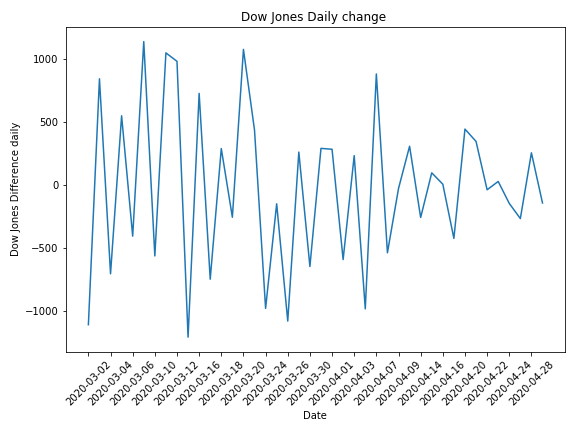
\includegraphics[width=0.45\textwidth]{images/dow_diff.png}\label{fig:diff}}
	\subfloat[Dow Jone Moving Average]{  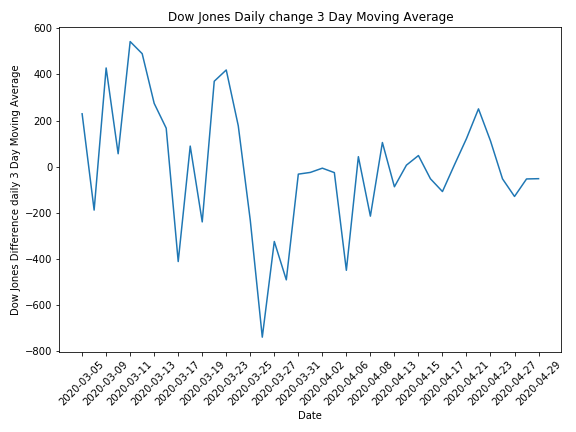
\includegraphics[width=0.45\textwidth]{images/dow_diff_ma.png}\label{fig:dow_diff_ma}}\\
	\caption{Dow Jones Daily Difference and Daily Difference Moving Average}
	\label{fig:dow_diff}
\end{figure}

Figure \ref{fig:avg_tone_diff} shows the daily Average tone of the events across days. Whilst this data is less chaotic than the Dow Jones data, the moving average for 3 days was still plotted and is shown in Figure \ref{fig:avg_ma}. It is immediately apparent that the Average Tone is always negative, which is perhaps to be expected given the frosty relationship between the USA and China during the months of March and April. What the moving average shows, is that the Dow Jones follows a slightly similar path throughout time, only a few dats later, as the trough in the moving average for the Dow Jones difference occurs a few days after the trough in the average tone.

\begin{figure}[H]
	\centering
	\subfloat[GDELT Average Tone]{  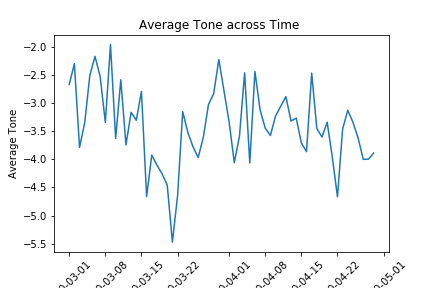
\includegraphics[width=0.45\textwidth]{images/avgtone.png}\label{fig:avg}}
	\subfloat[GDELT Average Tone 3 Day Moving Average]{  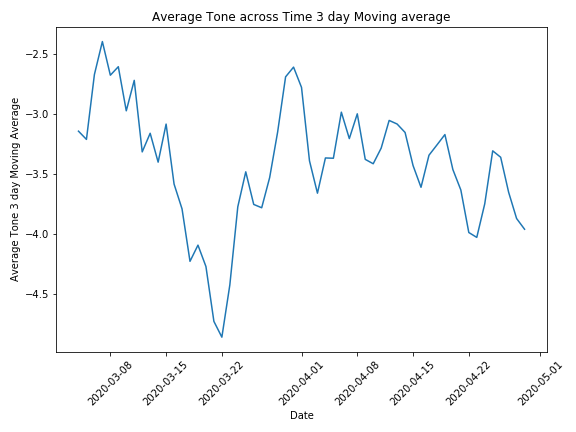
\includegraphics[width=0.45\textwidth]{images/avgtone_ma.png}\label{fig:avg_ma}}\\
	\caption{GDELT Average Tone over time and Moving Average}
	\label{fig:avg_tone_diff}
\end{figure}

Figure \ref{fig:gs_diff} shows the daily average of the Goldstein Scale of events across time, and as with the previous two plots, the 3 day moving average is shown in Figure \ref{fig:gs_ma}. The Goldstein Score, like the Dow Jones difference, appears to be chaotic, shifting from positive to negative fairly frequently. The moving average shows that there appears to be a peak halfway through the time period, followed by more fluctuation. 

\begin{figure}[H]
	\centering
	\subfloat[GDELT Goldstein Scale]{  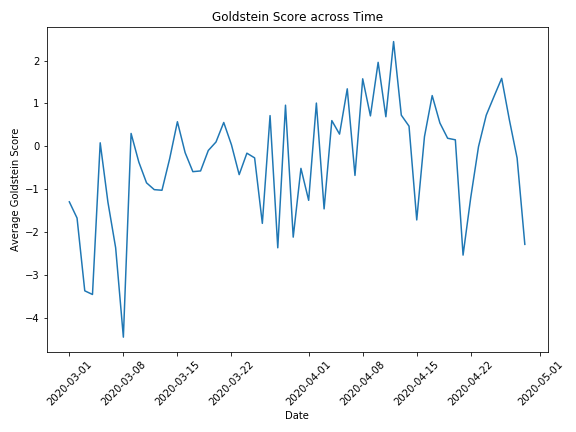
\includegraphics[width=0.45\textwidth]{images/goldsteinscore.png}\label{fig:gs}}
	\subfloat[GDELT Goldstein Scale 3 Day Moving Average]{  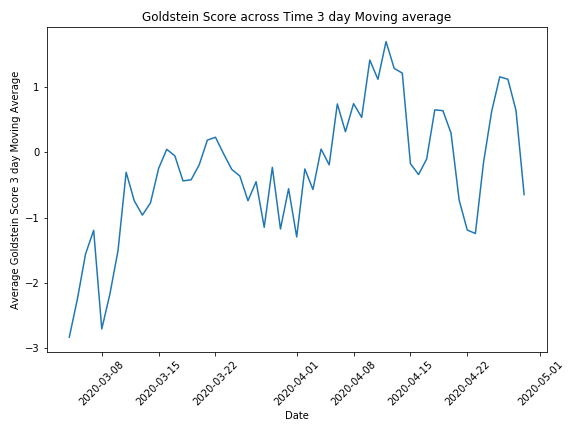
\includegraphics[width=0.45\textwidth]{images/goldsteinscore_ma.png}\label{fig:gs_ma}}\\
	\caption{GDELT Goldstein Scale over time and Moving Average}
	\label{fig:gs_diff}
\end{figure}

\subsection{Topic Modelling}
\subsubsection{TF-IDF}
The top Tf-idf terms are shown for the USA China data across the corpus in Figure \ref{fig:tfidfusachina}. This data was achieved by taking the average of the tfidf values across the entire dataset. The values are slightly lower, as there will be lots of tf-idf values of 0, where there are documents where the word doesn't exist. The 0 values of the Tf-Idf are included in the mean calculations as the parsing process for URLs is not perfect, and the Tf-Idf values can be non representative for some values if it was one of only 1 value present in the data.

\begin{figure}[H]
	\centering
	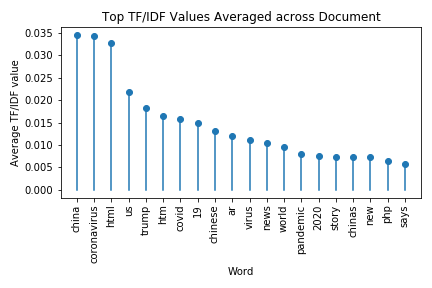
\includegraphics[width=0.49\textwidth]{Images/usa_stem_tfidf.png}
	\caption{Plot of the top 15 words which used TF-IDF in the USA/China specific data}
	\label{fig:tfidfusachina}
\end{figure}

Perhaps as expected, the most important and often occurring words are China and coronavirus.  Amongst the top words are also US, and Trump, along with variations of China and covid-19 and references to the pandemic. This is most interesting as a result, as something which no one had heard of prior to January/February dominated the news in March and April.

One of the other main words which pops up is html. This is most likely as a result of the fact that most of the URLs end with `.htm` or `.html`, and during the parsing html gets treated as a commonly occurring word. It was not removed as there could be legitimate stories which have the word in them. 

For the top values, the distribution of the tf-idf values across documents was calculated, excluding the 0 values. This is shown in Figure \ref{fig:tfidfdist}. The distributions are different to each other, but both follow a similar pattern in having a centre of the distribution be around a Tf-IDF value of around 0.25. One of the notable exceptions to this is the word `ar`, which is another error as a result of parsing. World and news both have a spike later on, but that is most likely due to the smaller sample size.

\begin{figure}[H]
	\centering
	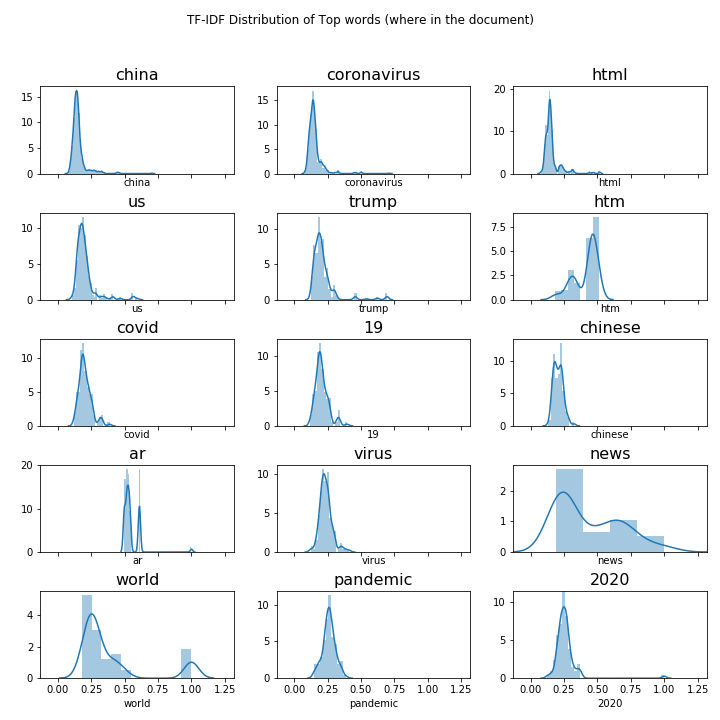
\includegraphics[width=0.49\textwidth]{Images/usa_tfidf_top_distribution.png}
	\caption{Distribution of the TF-IDF values across documents of the top 15 words (excluding documents where the Tf-IDF value was 0)}
	\label{fig:tfidfdist}
\end{figure}

\subsubsection{LDA}
\paragraph{Initial LDA}
Initially a topic model was run on one day's worth of Event data. The day was the 1st of November 2019. This was done as a reference point before running the LDA models on the specific USA/China chosen data.

There were two different topic models tried. Firstly one model with 3 topics was tried and then one model with 5 topics. The top words from each model are shown in word cloud format in Figures \ref{fig:single3wc} and \ref{fig:single5}. Alongside the word cloud, for each topics, the weight and the word count of the top words was also calculated and plotted. 
	
\begin{figure}[H]
	\centering
	\subfloat[Word Cloud 3 Topics]{  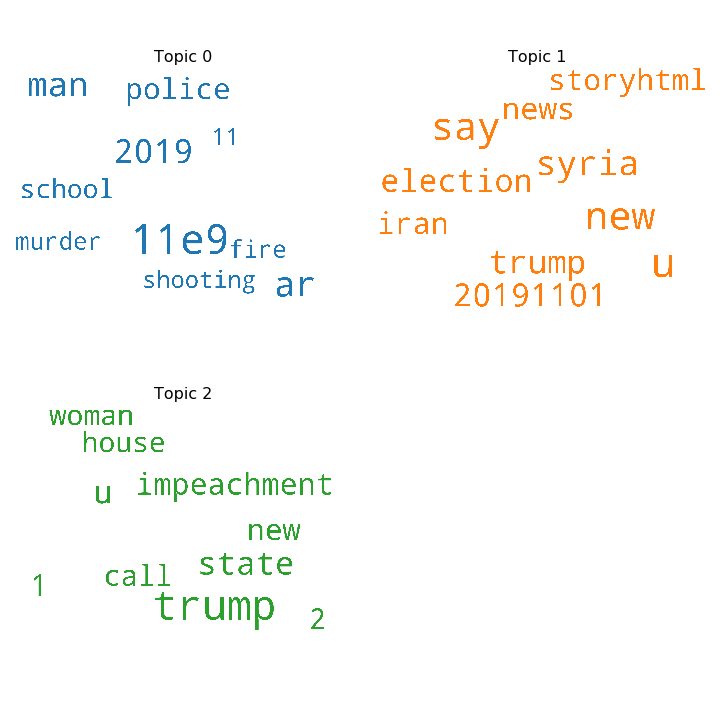
\includegraphics[width=0.8\textwidth]{images/single/word_cloud_single_3_topics.png}\label{fig:single3wc}}
\end{figure}
\begin{figure}[H]
	\centering
	\ContinuedFloat
	\subfloat[Word Weights 3 topics]{  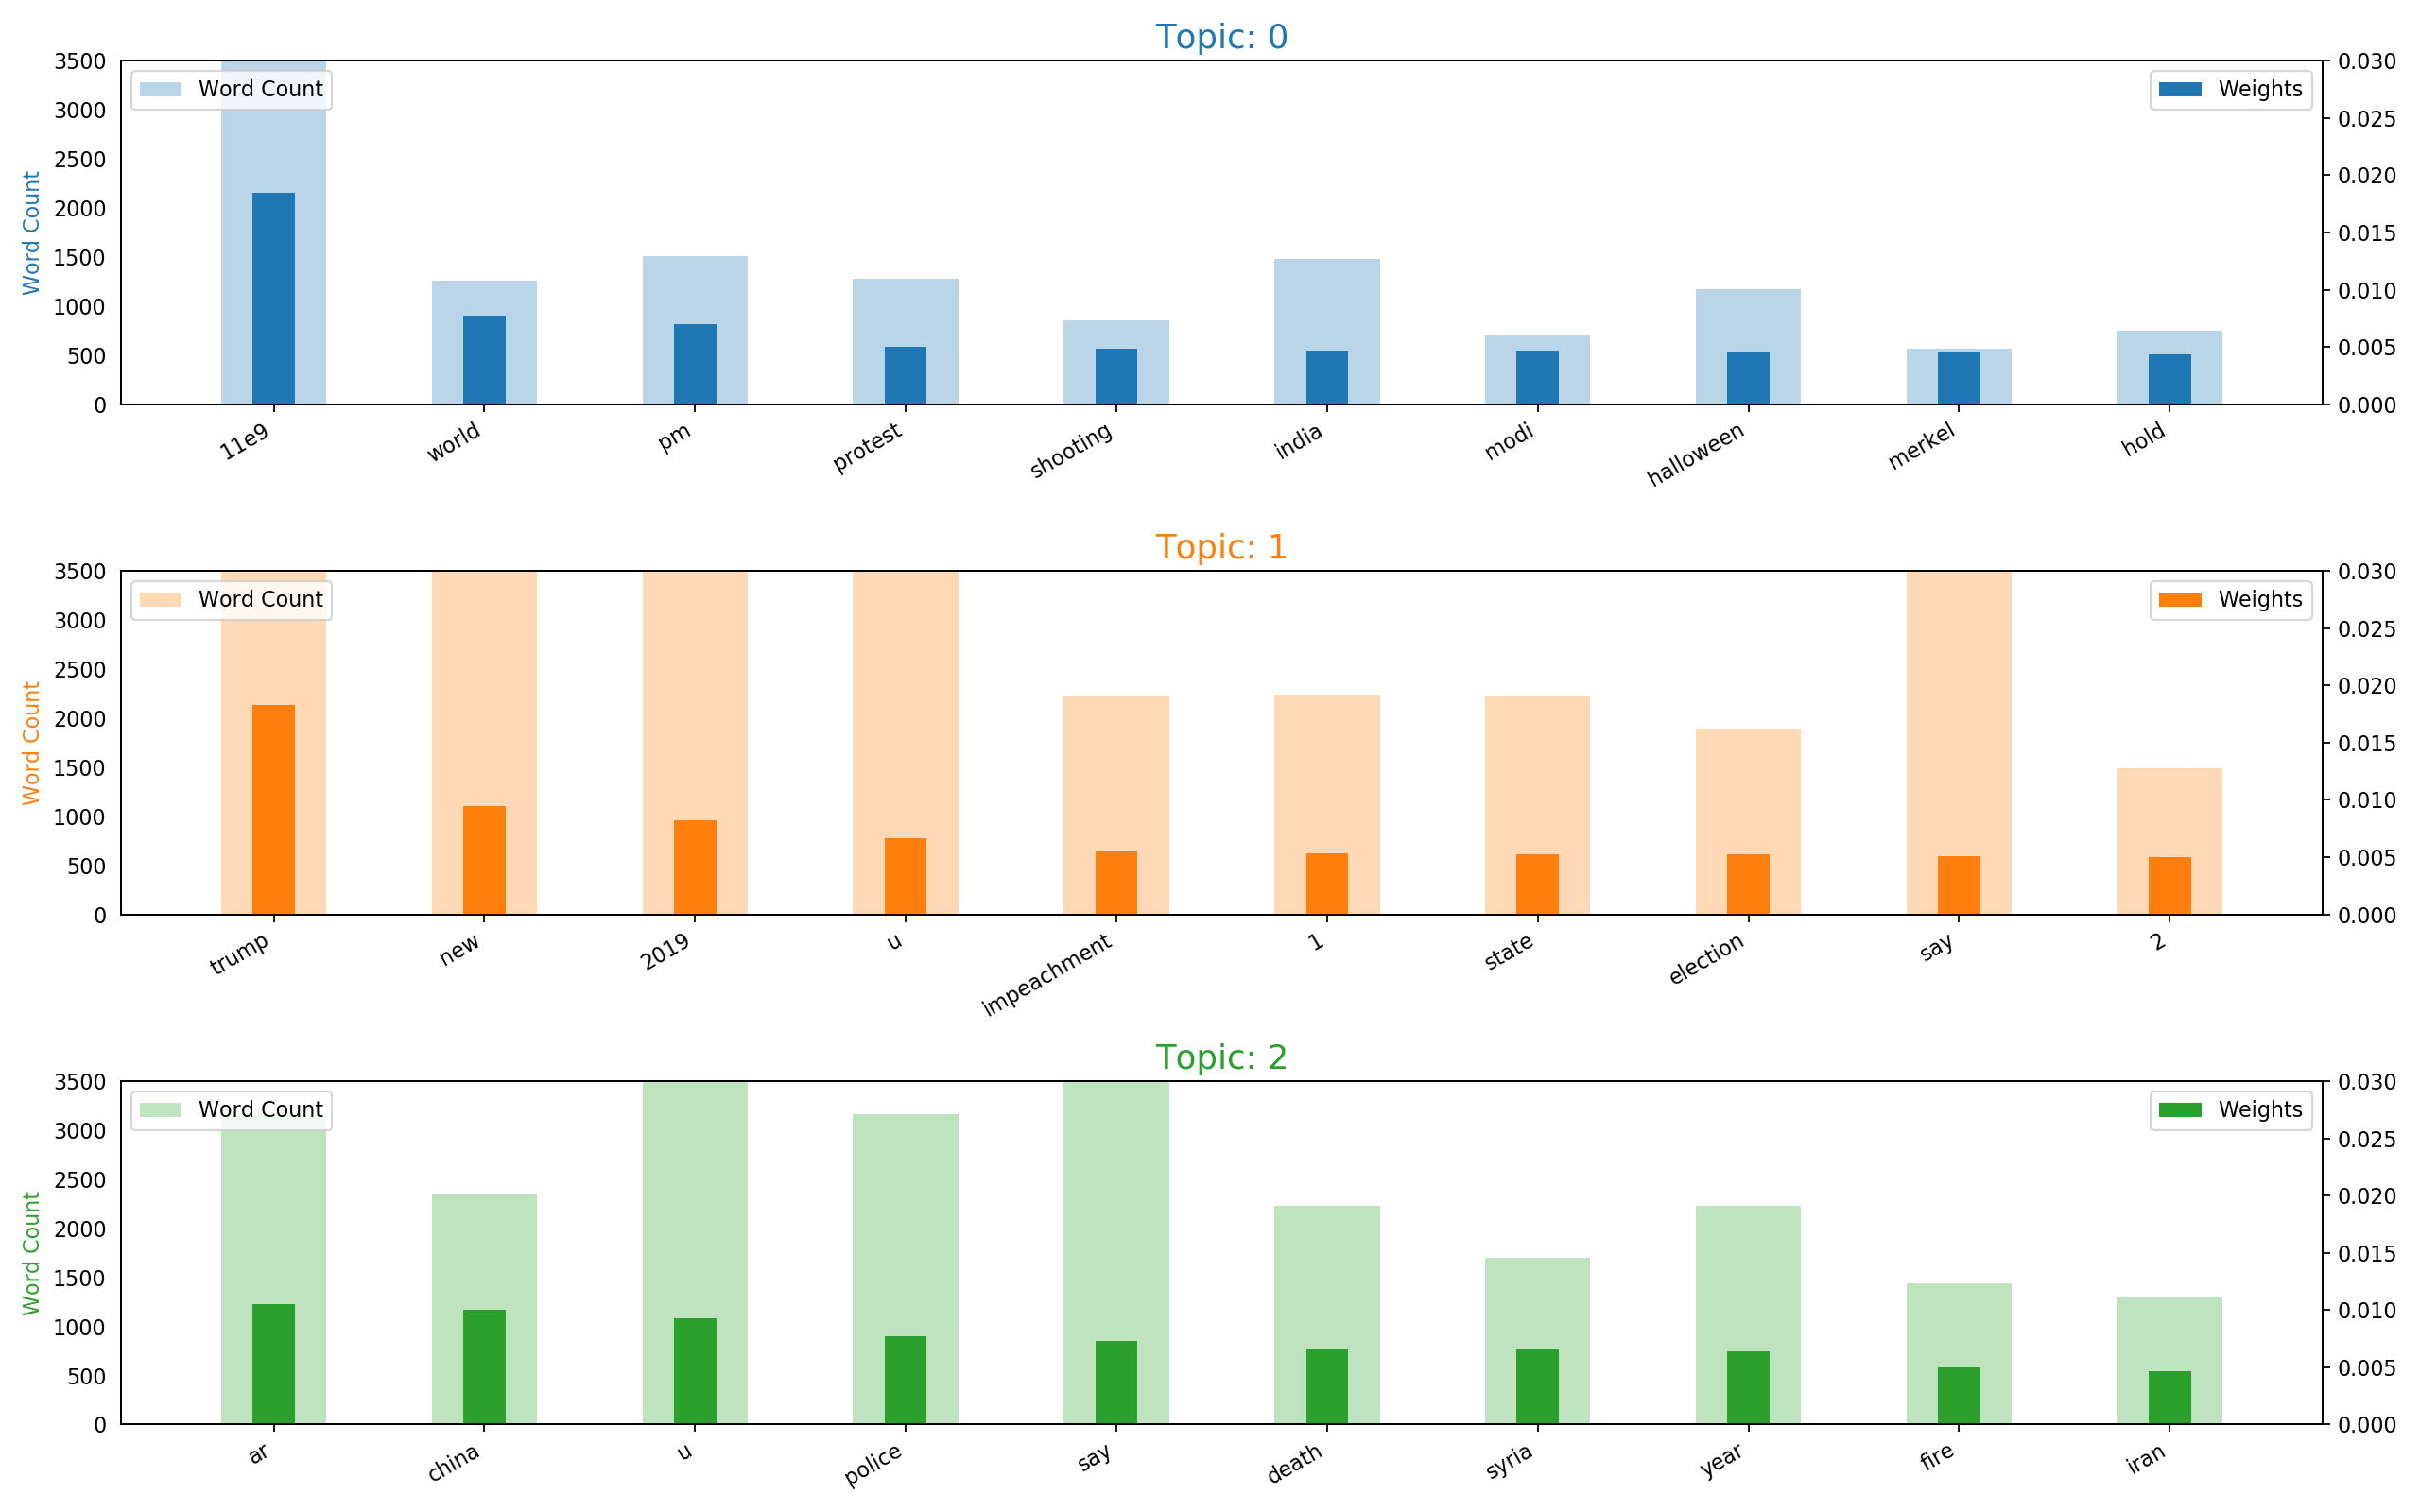
\includegraphics[width=0.8\textwidth]{images/single/word_weights_single_3_topics.png}\label{fig:single3ww}}\\
	
	\caption{Single Day Word Clouds for 5 topics}
	\label{fig:single3}
\end{figure}

Examining the word clouds for the model with three topics, there aren't any clear topics which are apparent. Topic 2 could vaguely be about the impeachment process for Donald Trump, Topic 0 appears to be focused on police brutality as a topic, and Topic 1 could broadly be referred to in terms of international news. Examining the Word importances, the main theme across topics ia that the word count is not the same as the word importance, in that some words have much higher occurrences, but lower weights and vice versa.

\begin{figure}[H]
	\centering
	\subfloat[Word Cloud 5 Topics]{  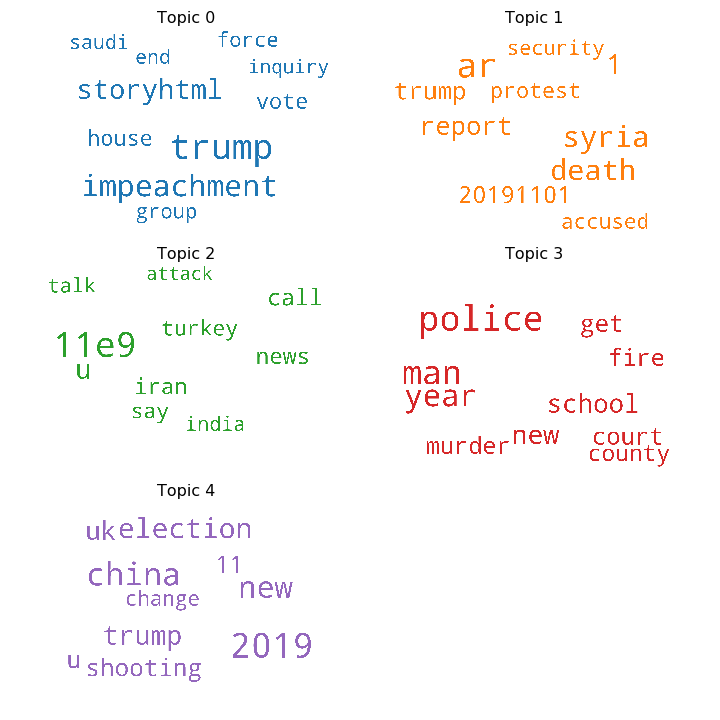
\includegraphics[width=0.8\textwidth]{images/single/word_cloud_single_5_topics.png}\label{fig:single5wc}}\\
	\subfloat[Word Weights 5 topics]{  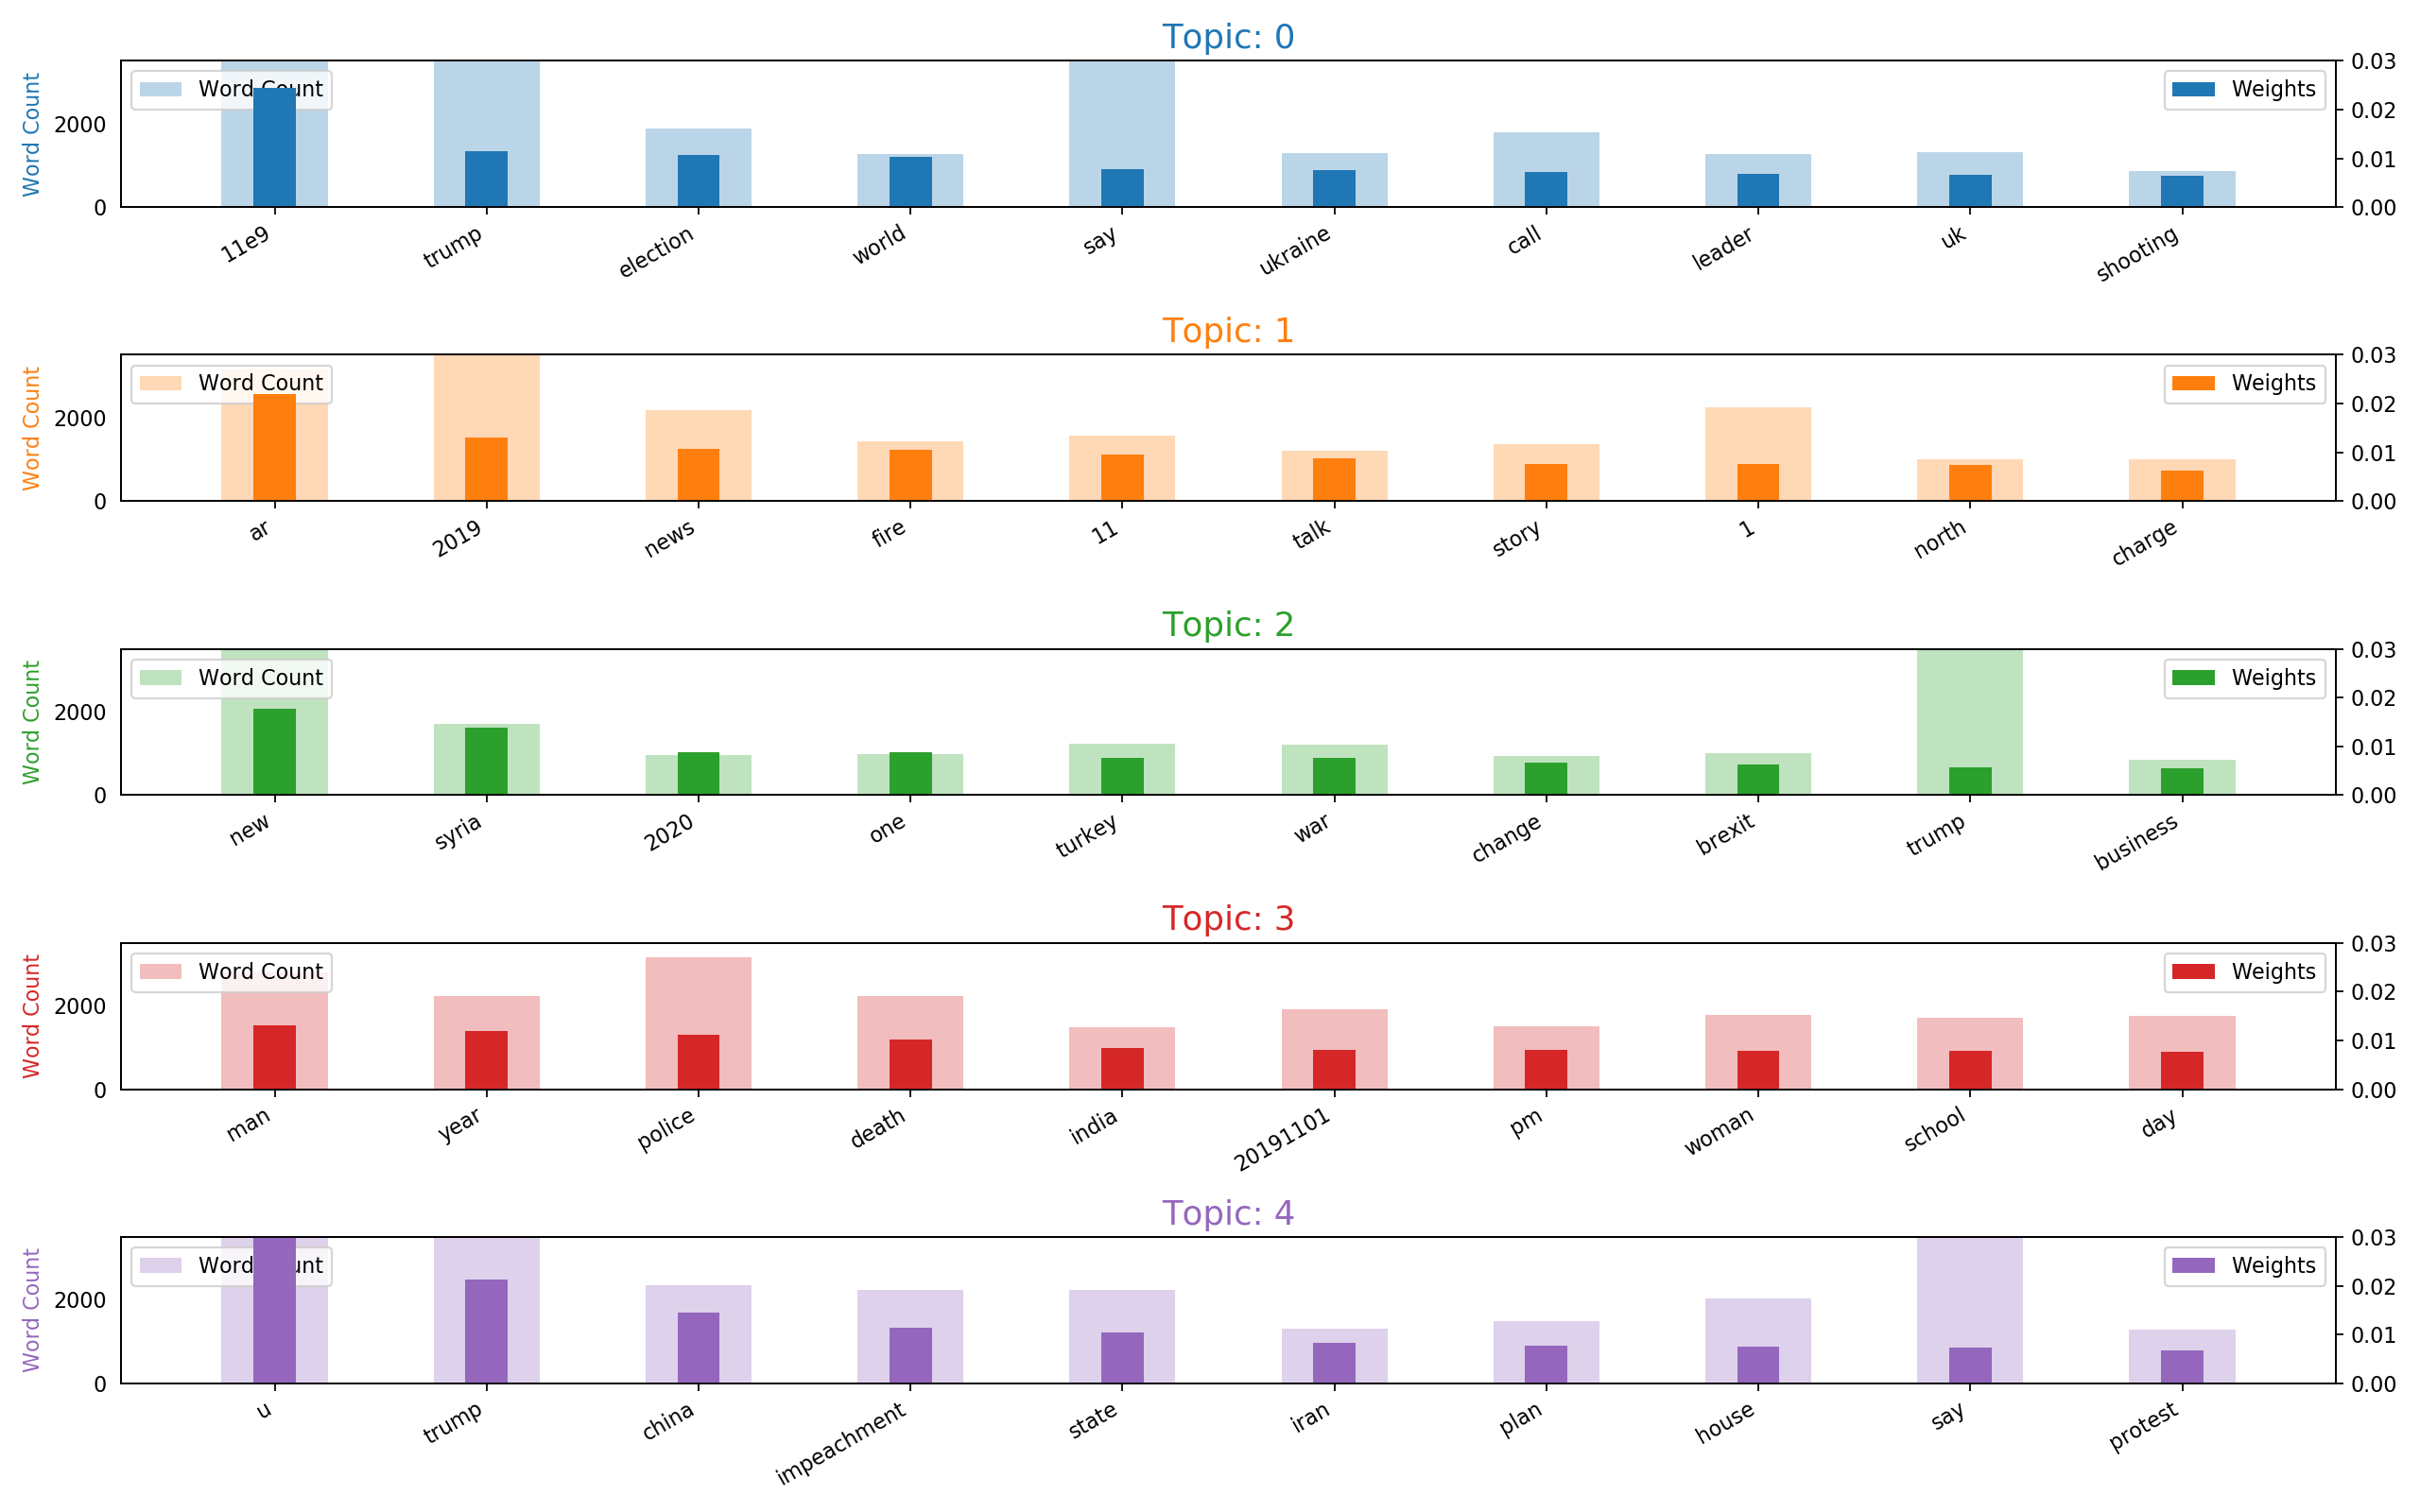
\includegraphics[width=1\textwidth]{images/single/word_weights_single_5_topics.png}\label{fig:single5ww}}\\
	
	\caption{Single Day Word Clouds for 5 topics}
	\label{fig:single5}
\end{figure}	

Examining the 5 topic model, the topics are much closer together, its very difficult to find a central topic for each topic, topic 3 could potentially be about police and court information, but aside from that there does not appear to any coherency otherwise, with words like Trump being in multiple topics and international countries spread across topics. The word importance and weight plot also doesn't reveal anything new, like the previous model, the word's count is not related to the importance and perhaps expectedly, the words in the topics are not related to each other.

\paragraph{USA/China Data}
A similar procedure was used for the USA/China data, but models with 2, 3, and 4 topics each were tried. The word clouds of the results and the subsequent word importances to each topic are shown in Figures \ref{fig:usa2}, \ref{fig:usa3}, and \ref{fig:usa2}. 
\begin{figure}[H]
	\centering
	\subfloat[USA/China Word Cloud 2 Topics]{  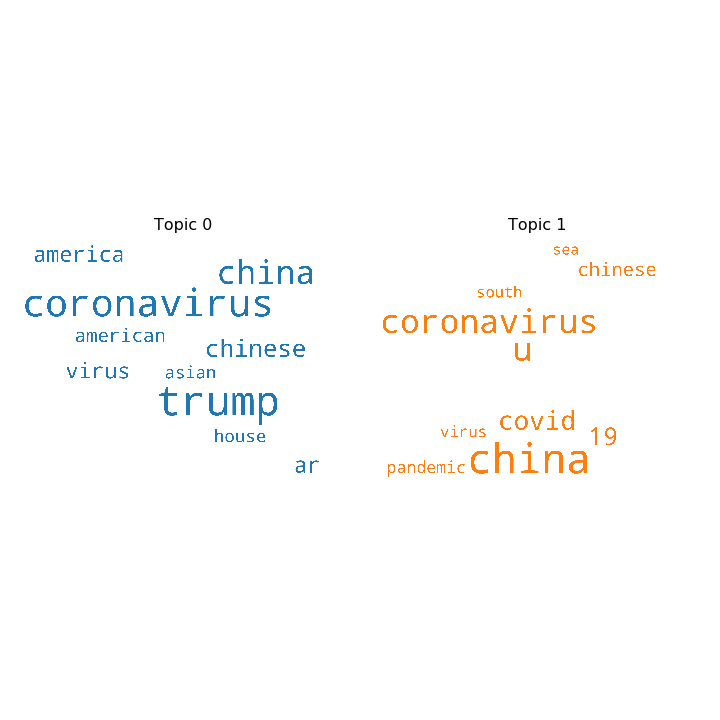
\includegraphics[width=0.6\textwidth]{images/uschina/word_cloud_usa_2_topics.png}\label{fig:us2wc}}\\
	\subfloat[USA/China Word Weights 2 topics]{  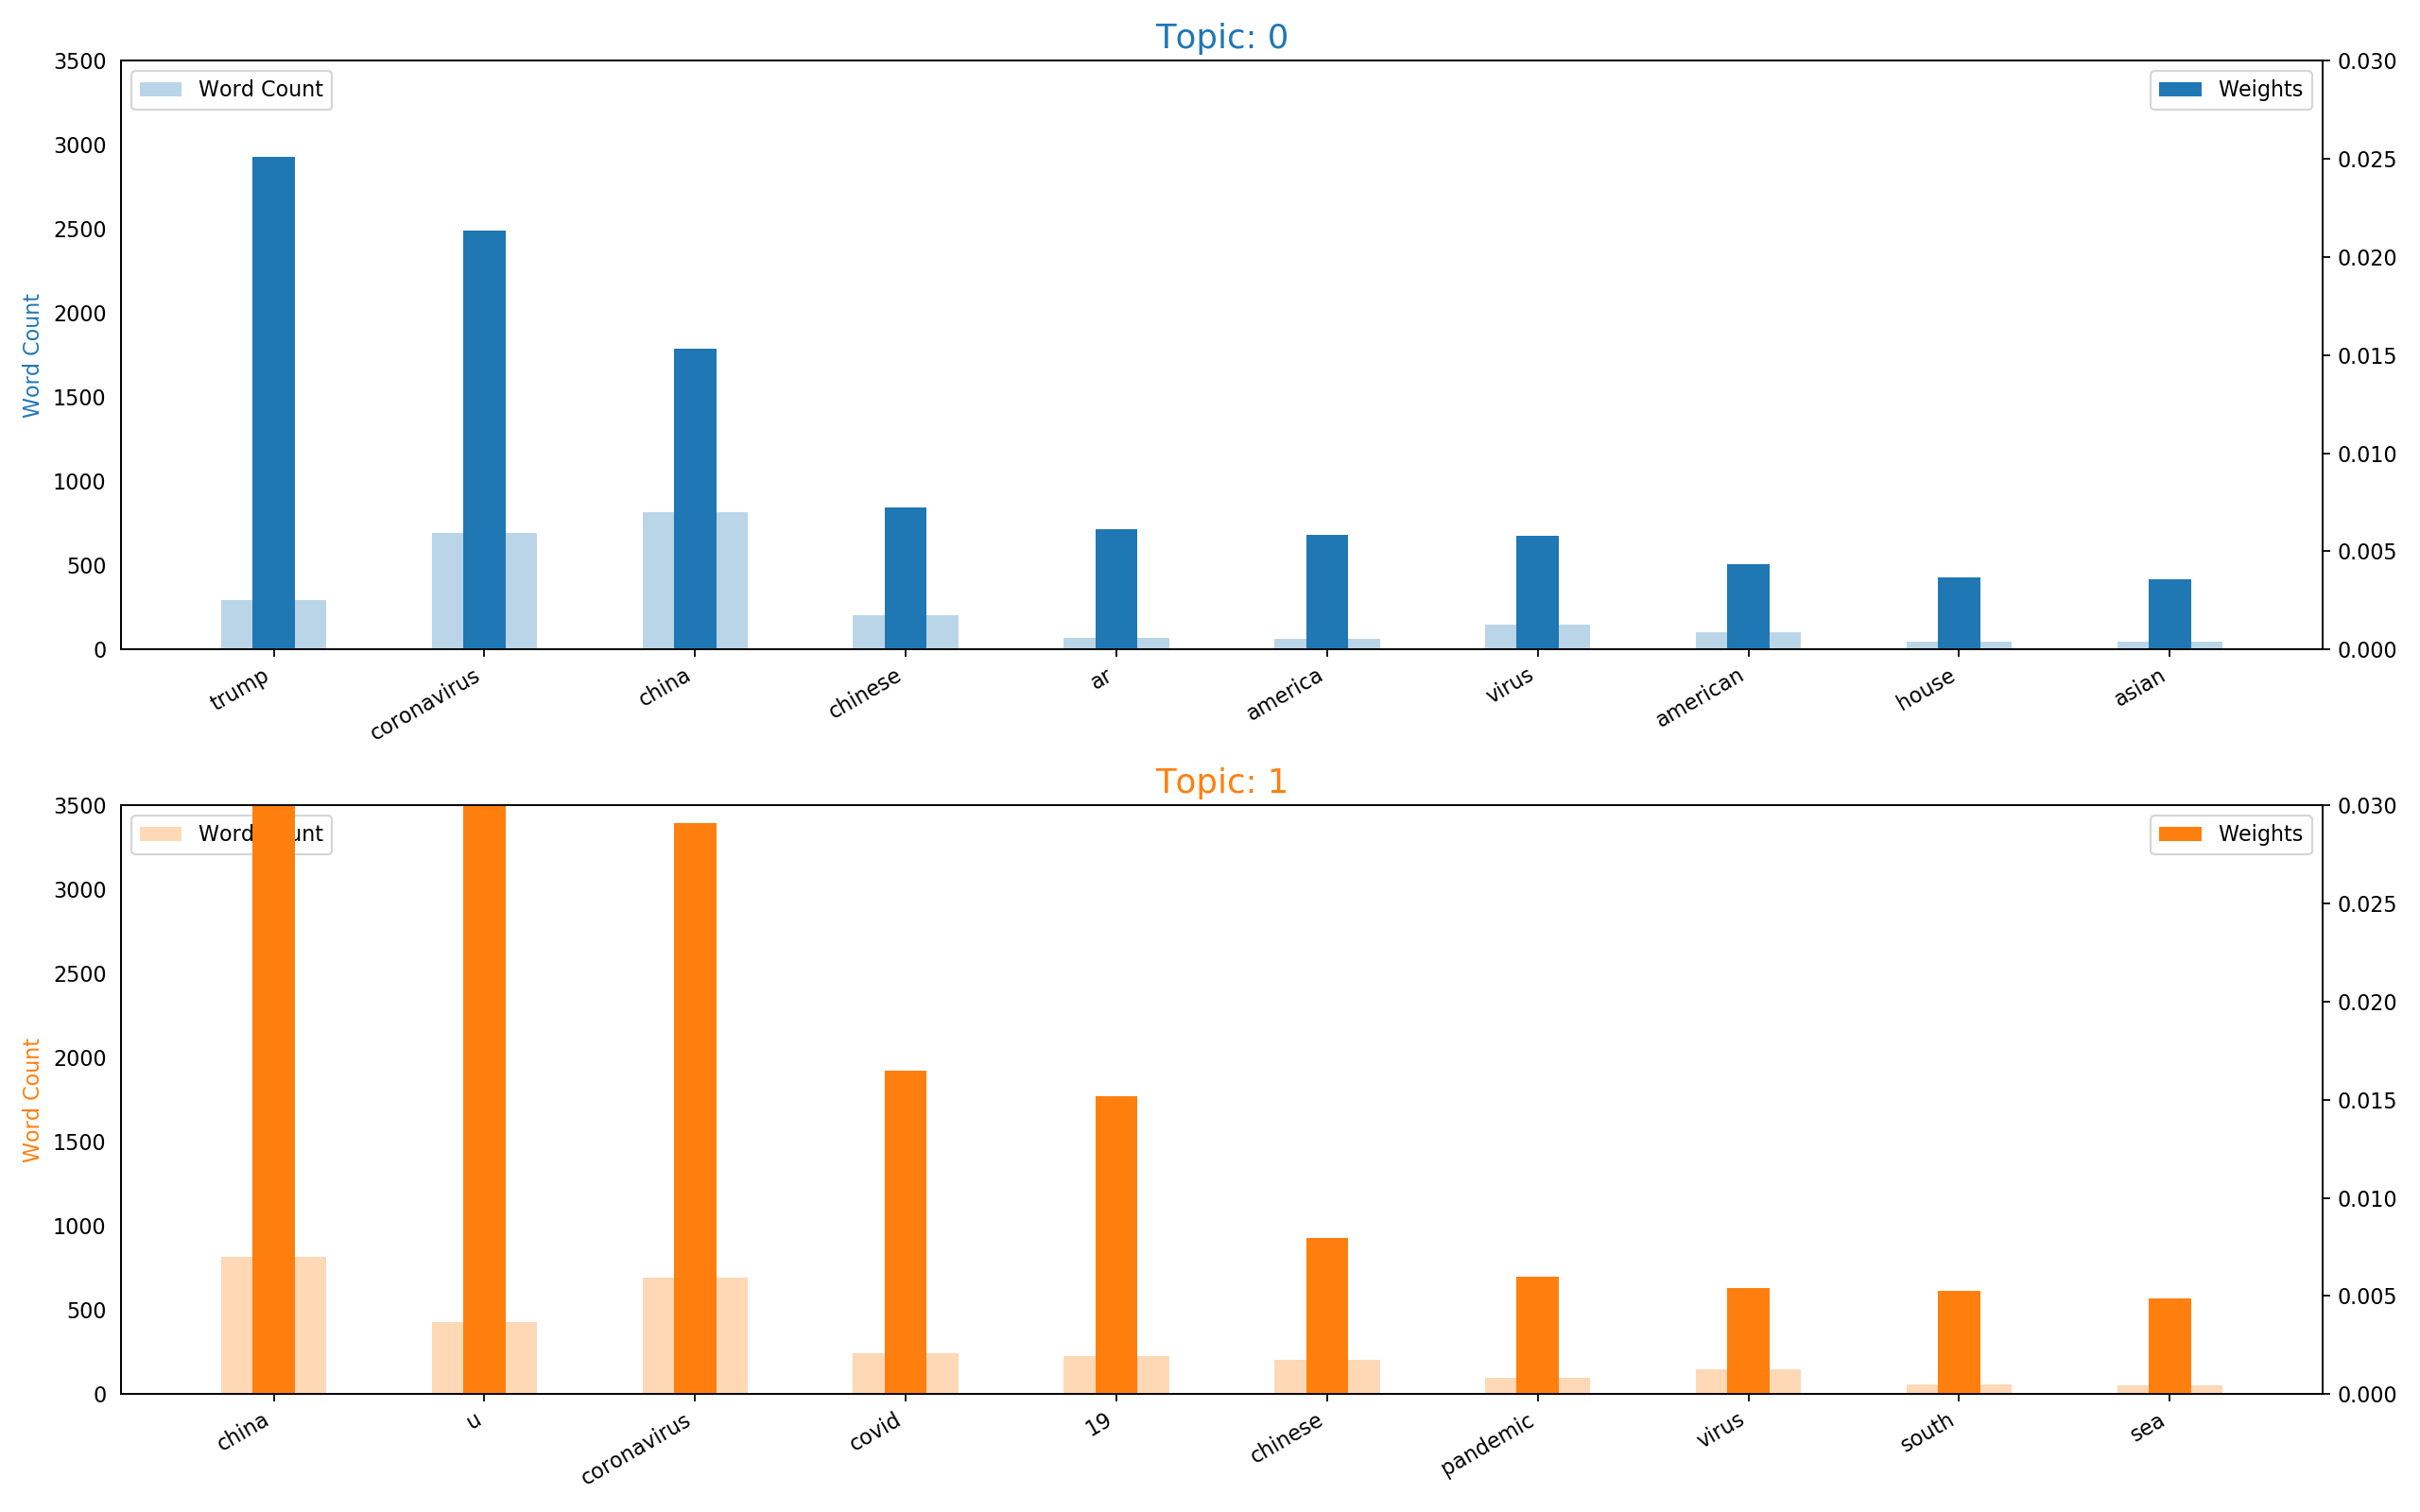
\includegraphics[width=0.8\textwidth]{images/uschina/word_weights_usa_2_topics.png}\label{fig:us2ww}}\\
	
	\caption{USA/China Word Clouds for 2 topics}
	\label{fig:usa2}
\end{figure}
Examining the first LDA model which had 2 topics on the USA China data, the themes are very similar. Words related to the pandemic, and words such as China and Trump appear in both topics, which suggest the model hasn't been effective in differentiating between the topics effectively. Looking at the word weights in Figure \ref{fig:us2ww}, for all of the words, the weights are all higher than the word counts. The highest word weights are Trump, Coronavirus, China and China, Coronavirus, and `u`. `U` appears appears to be another issue with the parsing.  
\begin{figure}[H]
	\centering
	\subfloat[USA/China Word Cloud 3 Topics]{  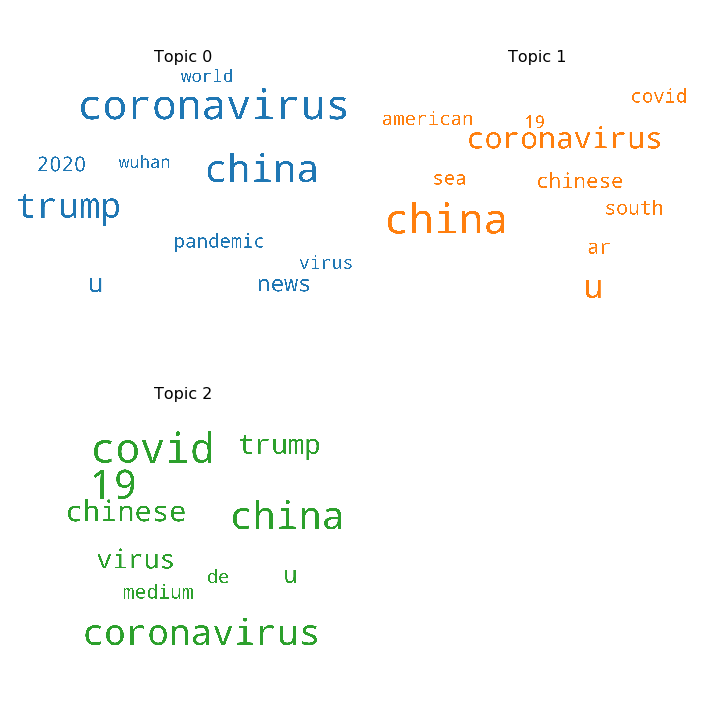
\includegraphics[width=0.6\textwidth]{images/uschina/word_cloud_usa_3_topics.png}\label{fig:us3wc}}\\
	\subfloat[USA/China Word Weights 3 topics]{  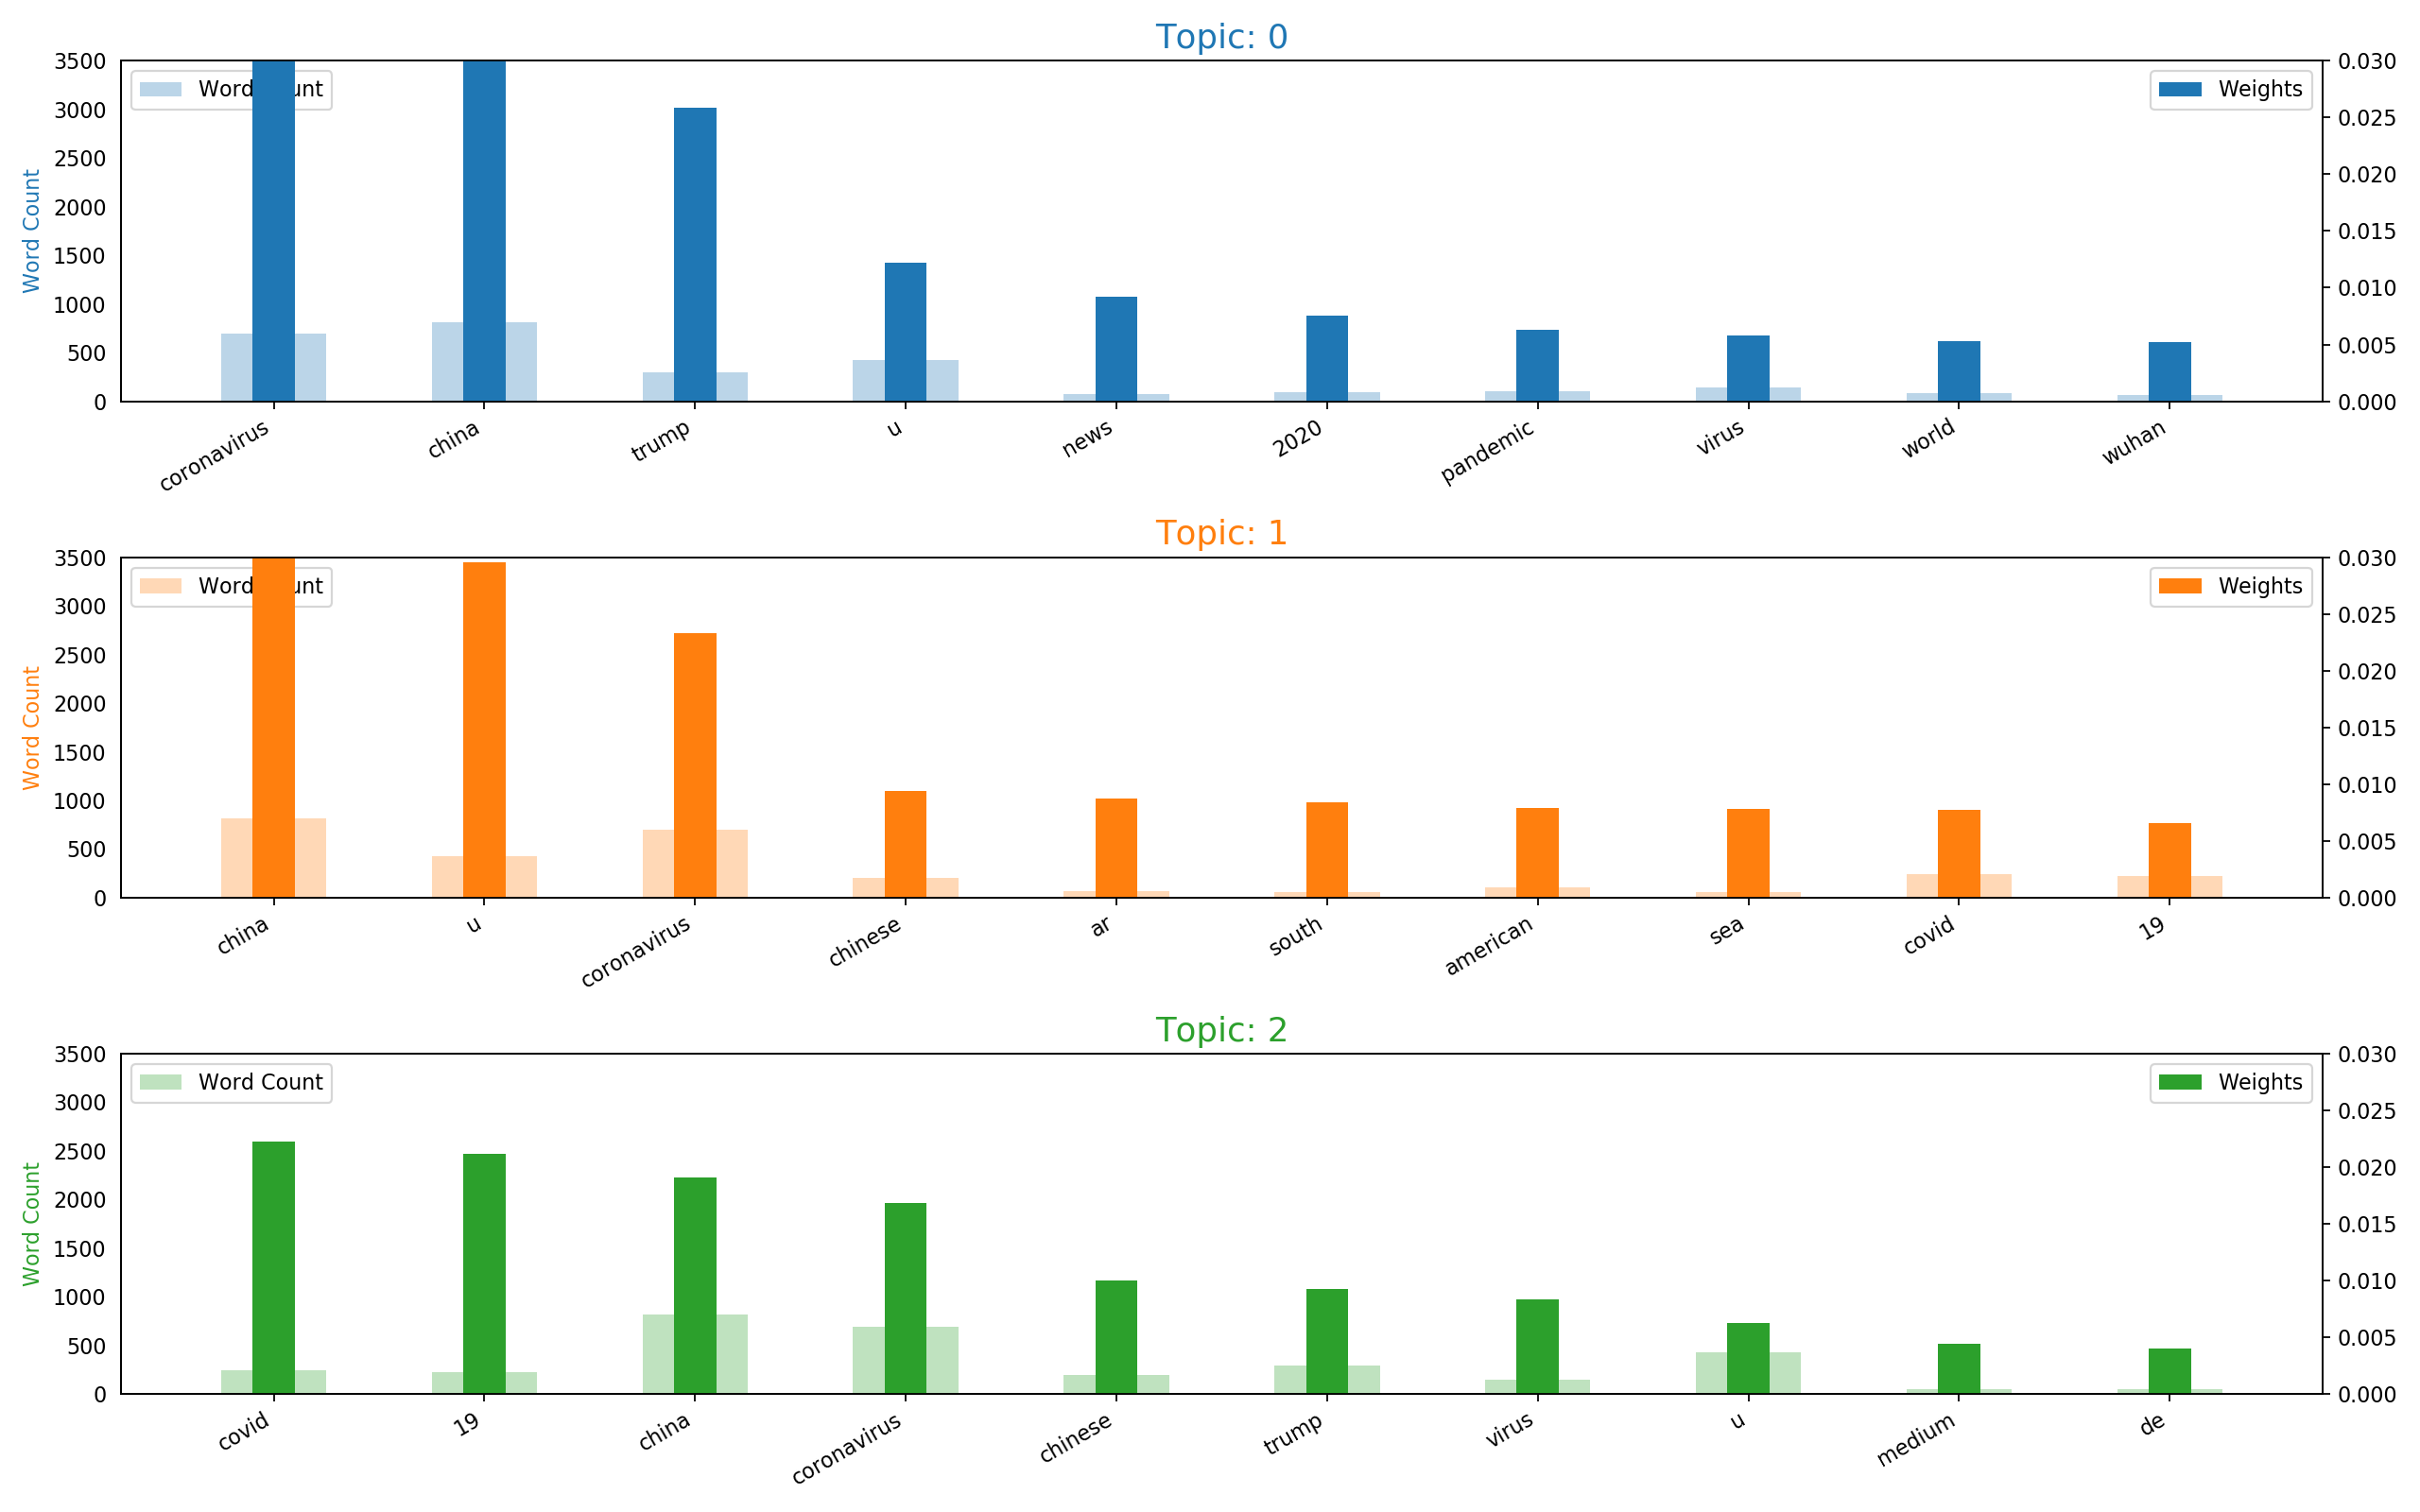
\includegraphics[width=0.8\textwidth]{images/uschina/word_weights_usa_3_topics.png}\label{fig:us3ww}}\\
	
	\caption{USA/China Word Clouds for 3 topics}
	\label{fig:usa3}
\end{figure}

Looking the the three topic model, the topics are even closer together than the two topic model. The main words as before appear in all of the topics, suggesting the topic model hasn't separated any topics well. The word weights are also similar to the two topic model. One of the differences between the two topic and the three topic model is the 3rd topic weights are noticeably smaller than the first and second topics. 

\begin{figure}[H]
	\centering
	\subfloat[USA/China Word Cloud 4 Topics]{  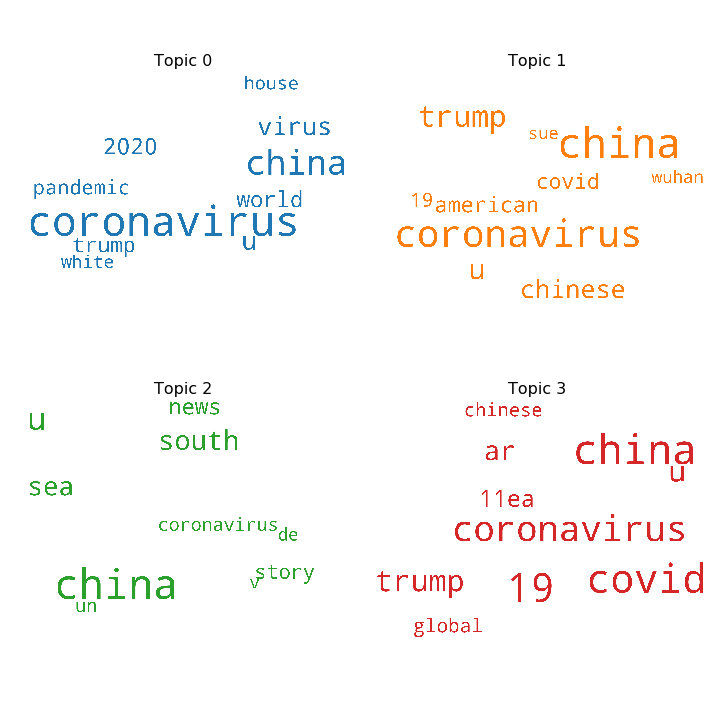
\includegraphics[width=0.6\textwidth]{images/uschina/word_cloud_usa_4_topics.png}\label{fig:us4wc}}\\
	\subfloat[USA/China Word Weights 4 topics]{  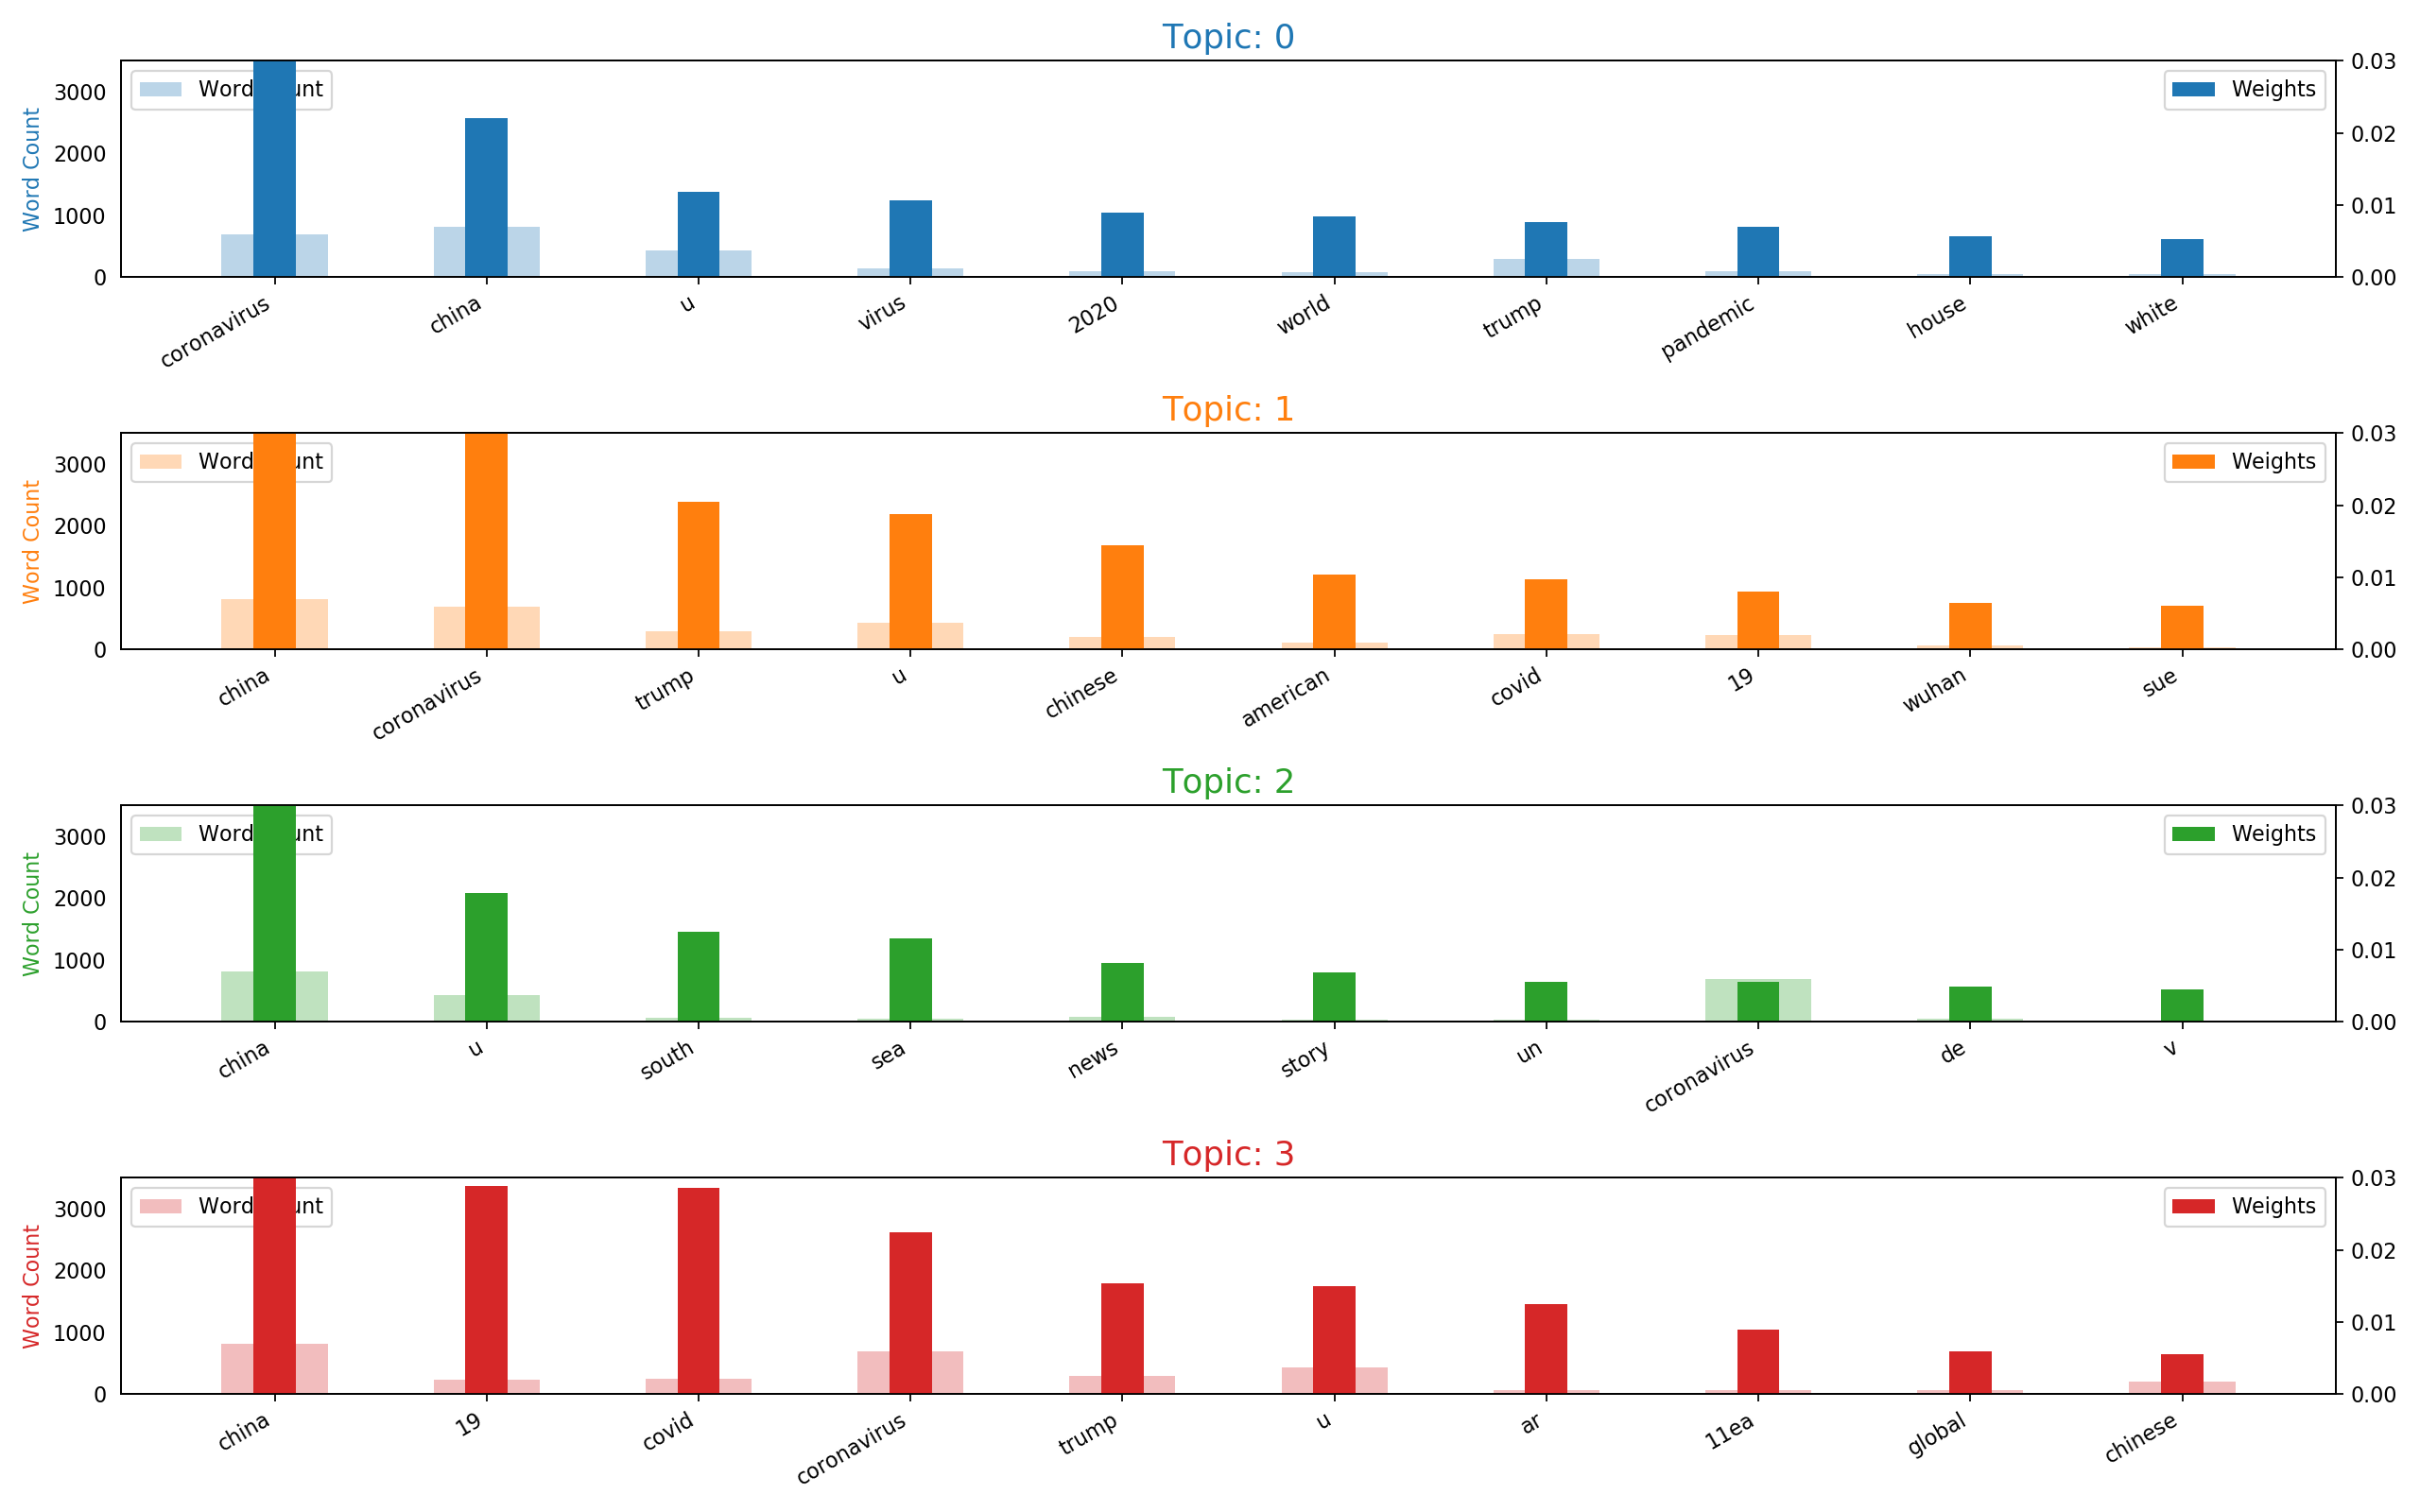
\includegraphics[width=0.8\textwidth]{images/uschina/word_weights_usa_4_topics.png}\label{fig:us4ww}}\\
	
	\caption{USA/China Word Clouds for 4 topics}
	\label{fig:usa4}
\end{figure}

The 4 topic model behaves in a similar manner to the previous 2 topic models. the main words are split across the 4 topics with no real distinction between the topics present. 

\subsubsection{K Means}
Similar to the LDA models, the K-means was tried with 2, 3, and 4 clusters. The word cloud of the top words are shown in Figures \ref{fig:wck2}, \ref{fig:wck3}, and \ref{fig:wck4}. Alongside the word clouds, the clusters were decomposed into 2 and 3 dimensions by both Principal Component Analysis (PCA) and T-distributed Stochastic Neighbour Embedding (T-SNE). This was to see whether the clusters had been successful in separating the data at any level. This is shown for the different number of cluster in Figures \ref{fig:k2pca}, \ref{fig:k3pca}, and \ref{fig:k4pca} respectively. Furthermore, the Mahalanobis and Euclidean distances were plotted for all of the points associated with a cluster for all of the clusters present. This is shown in Figures \ref{fig:distk2}, \ref{fig:distk3}, and \ref{fig:distk4} respectively. 

To compare the efficacy of clusters in being able to filter information, the Mahalanobis distance from centre of clusters for variety of phrases as calculated, and plotted in Figures \ref{fig:wordsk2}, \ref{fig:wordsk3}, and \ref{fig:wordsk4}, alongside the distribution of points for each cluster. For all of the Mahalanobis distances, the phrases were several orders of magnitude out from the distribution of points for each cluster, so the results had to be logged before being plotted.  
\paragraph{Clustering with k=2}
\begin{figure}[H]
	\centering
	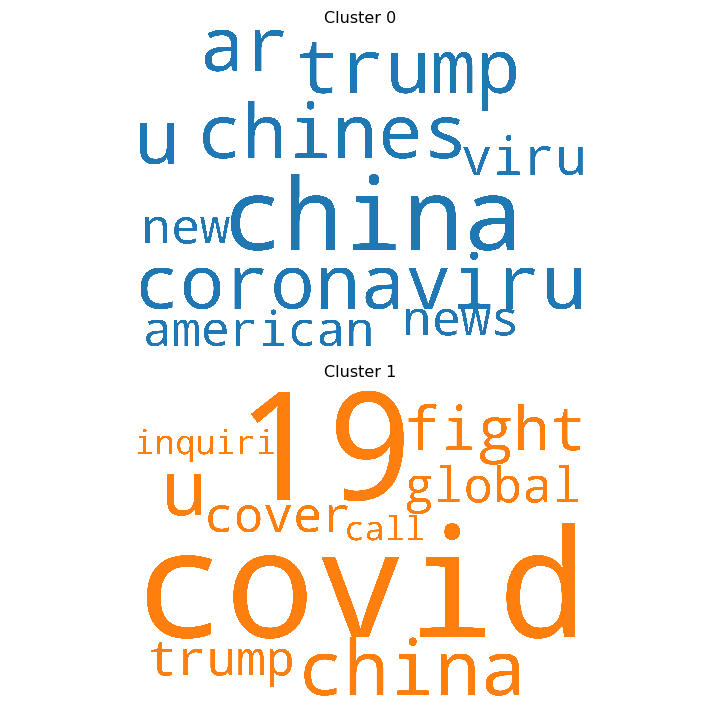
\includegraphics[width=0.8\textwidth]{images/kmeans_word_cloud_k=2.png}
	\caption{Word Cloud for k=2 clusters}
	\label{fig:wck2}
\end{figure}
Examining the word cloud created for a two cluster model, a similar picture appears as with the LDA models. There are several words which are close to both of the clusters, which, in a similar fashion to the LDA model, mean that any topics present are not being differentiated. This is evident in Figure \ref{fig:k2pca}, in which both T-SNE and PCA in both 2 and 3 dimensions show that the clusters are not distinct from each other. Interestingly, both the 2d and 3D PCA plots, Figures \ref{fig:pca2k2} and \ref{fig:pca2k3}, appear to show clean boundaries, however, it is not the most obvious of cluster definitions.

\begin{figure}[H]
	\centering
	\subfloat[2D PCA k=2]{  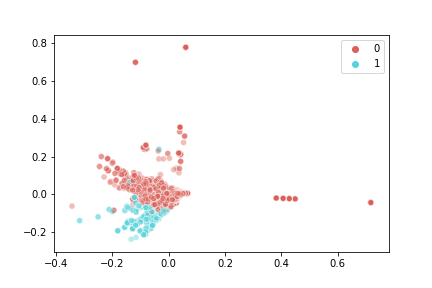
\includegraphics[width=0.45\textwidth]{images/kmeans_2d_pca_k=2.png}\label{fig:pca2k2}}
	\subfloat[3D PCA k=2]{  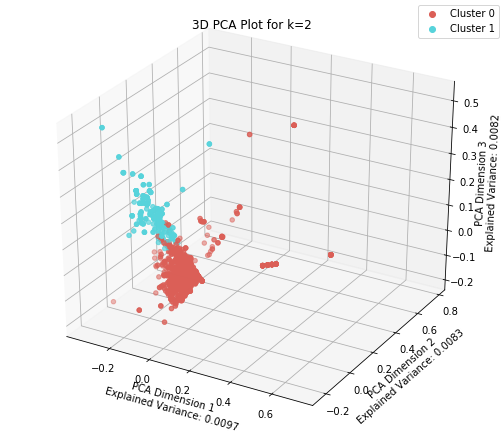
\includegraphics[width=0.45\textwidth]{images/kmeans_3d_pca_k=2.png}\label{fig:ts2k2}}\\
	\subfloat[2D T-SNE k=2]{  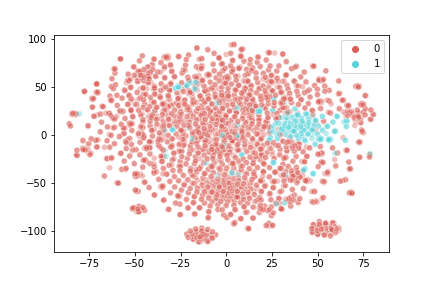
\includegraphics[width=0.45\textwidth]{images/kmeans_2d_tsne_k=2.png}\label{fig:pca3k2}}
	\subfloat[3D T-SNE k=2]{  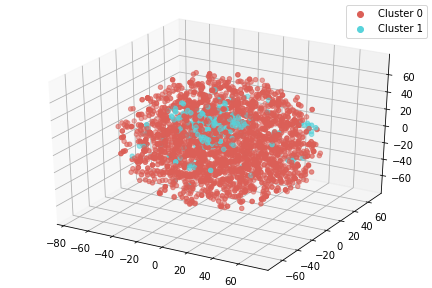
\includegraphics[width=0.45\textwidth]{images/kmeans_3d_tsne_k=2.png}\label{fig:ts3k2}}\\
	\caption{Decompositions of the clusters in 2 and 3 dimensions using PCA and T-SNE for k=2}
	\label{fig:k2pca}
\end{figure}
Examining the Mahalanobis distances for the two clusters, there doesn't appear to be any noticeable pattern, the distributions are slightly bimodal, compared to the Euclidean distances, which are much more normally distributed. The majority of points are associated with cluster 0, with the rest going to Cluster 1.
\begin{figure}[H]
	\centering
	\subfloat[Mahalanobis Distance]{  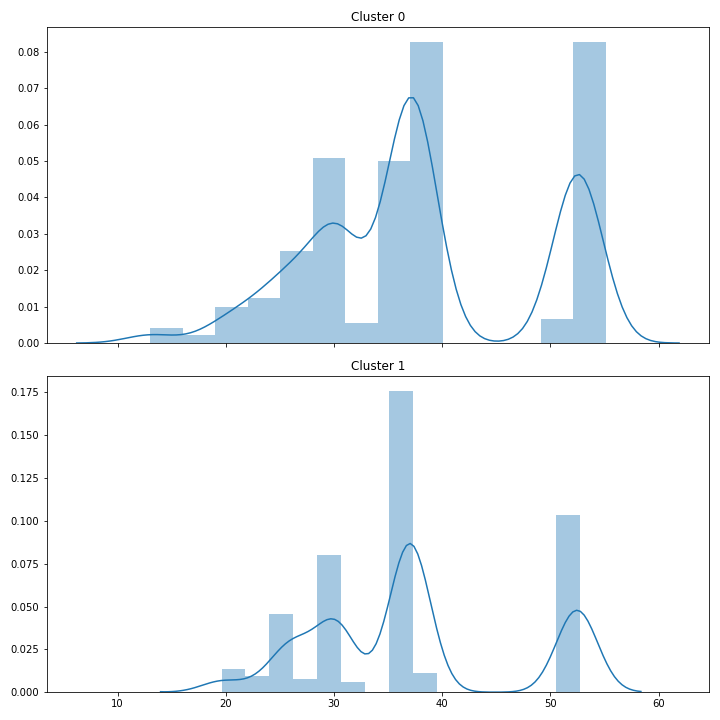
\includegraphics[width=0.45\textwidth]{images/kmeans_mahalanobis_distance_k=2.png}\label{fig:mhk2}}
	\subfloat[Euclidean Distances]{  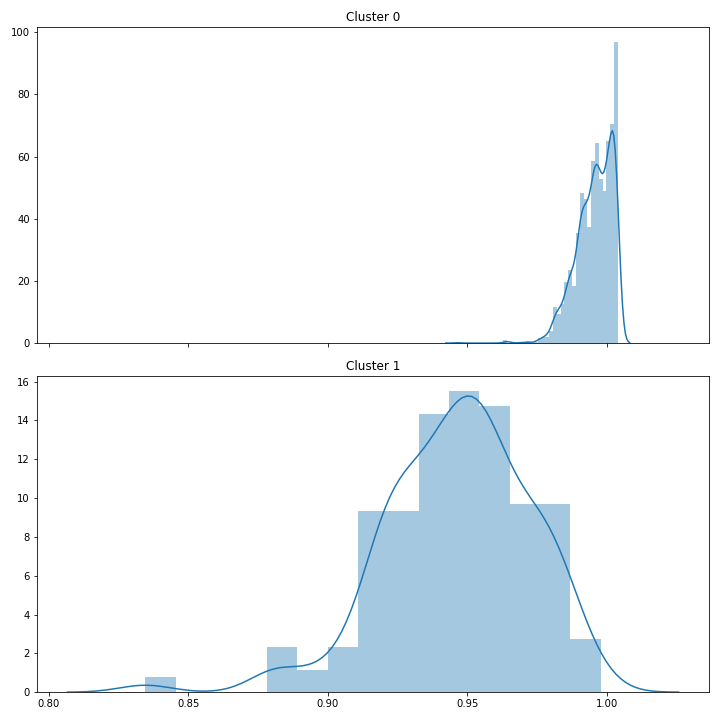
\includegraphics[width=0.45\textwidth]{images/kmeans_euclidean_distance_k=2.png}\label{fig:euk2}}\\
	
	\caption{Cluster Distances (Mahalanobis and Euclidean) for k=2 clusters}
	\label{fig:distk2}
\end{figure}

Comparing the results plotted on the log scale shown in Figure \ref{fig:wordsk2}, the first thing which becomes apparent is that the distances for the words appears to be the same between clusters, i.e. all phrases tested are equally far from both cluster 0 and cluster 1, this is perhaps unsurprising as the distance from the both clusters is extremely large. Comparing the words themselves, aside from the individual word `covid`, the phrases are fairly close together, with what appears to be two sets of lines. The first lines are the `coronavirus hits remote utah`, and the `aboriginal peoples australia complain` with the remainder of the headlines making up the remainder of the lines, nearly all of the results are between 27 and 28.  
\begin{figure}[H]
	\centering
	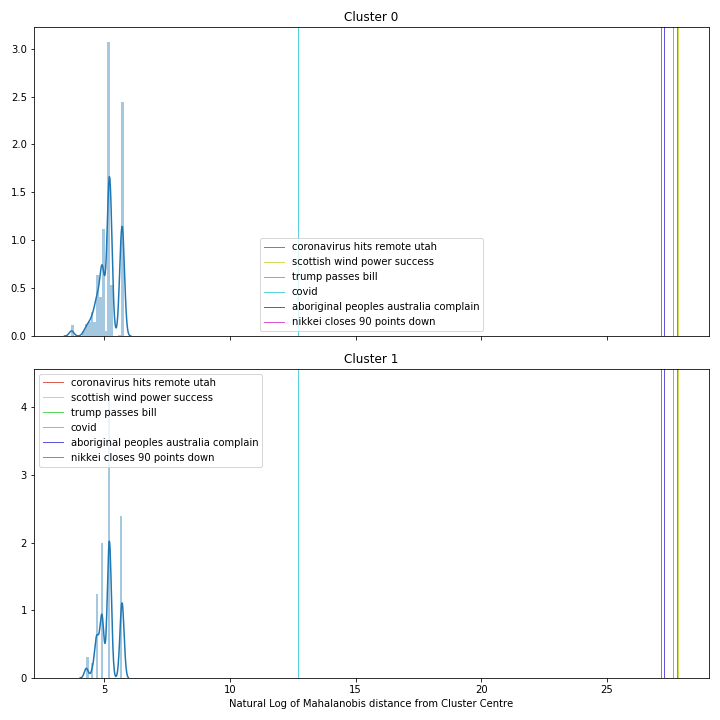
\includegraphics[width=0.8\textwidth]{images/words_kmeans_mahalanobis_distance_k=2.png}
	\caption{Log of Mahalanobis Distances for Clusters and Selected Phrases for k=2 clusters}
	\label{fig:wordsk2}
\end{figure}

\paragraph{Clustering when k=3} 
Examining the word cloud when there are 3 clusters, all of the clusters are similar to the k=2, in that they have very similar topics related to China and the Covid 19 Pandemic. Examining the decomposition plots, the clusters are close together, and the cluster definitions do not appear to be definitively useful. There are two smaller clusters present, which potentially could be clusters, but when examined, they represented a mixture of parsing errors from URLs, and numbers and letter combinations left over from URL parsing.  
\begin{figure}[H]
	\centering
	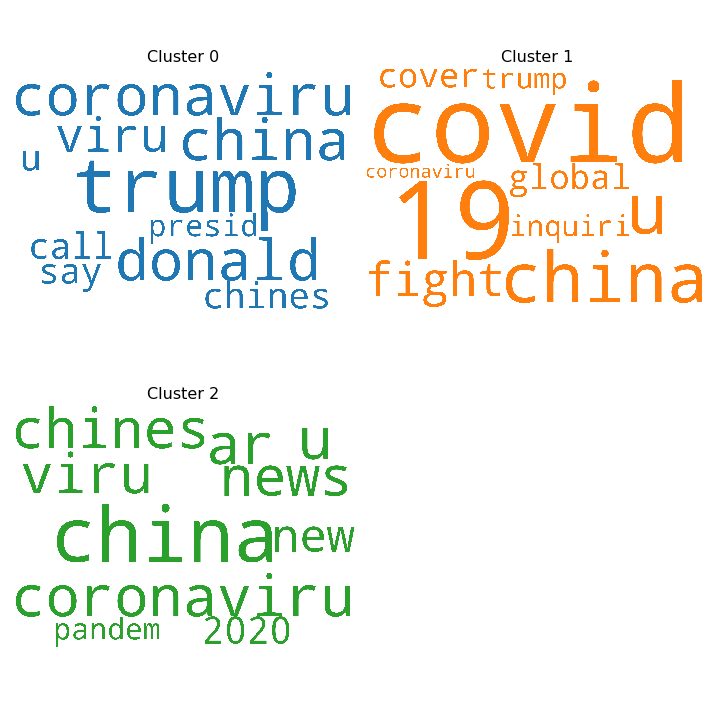
\includegraphics[width=0.8\textwidth]{images/kmeans_word_cloud_k=3.png}
	\caption{Word Cloud for k=3 clusters}
	\label{fig:wck3}
\end{figure}

\begin{figure}[H]
	\centering
	\subfloat[2D PCA k=3]{  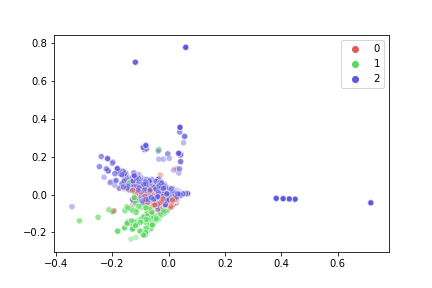
\includegraphics[width=0.45\textwidth]{images/kmeans_2d_pca_k=3.png}\label{fig:pca2k3}}
	\subfloat[3D PCA k=3]{  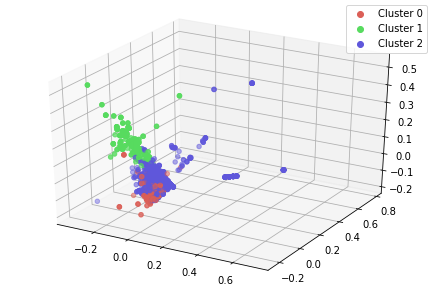
\includegraphics[width=0.45\textwidth]{images/kmeans_3d_pca_k=3.png}\label{fig:ts2k3}}\\
	\subfloat[2D T-SNE k=3]{  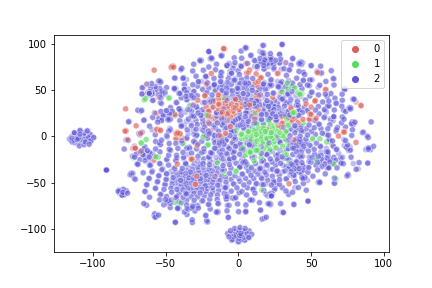
\includegraphics[width=0.45\textwidth]{images/kmeans_2d_tsne_k=3.png}\label{fig:pca3k3}}
	\subfloat[3D T-SNE k=3]{  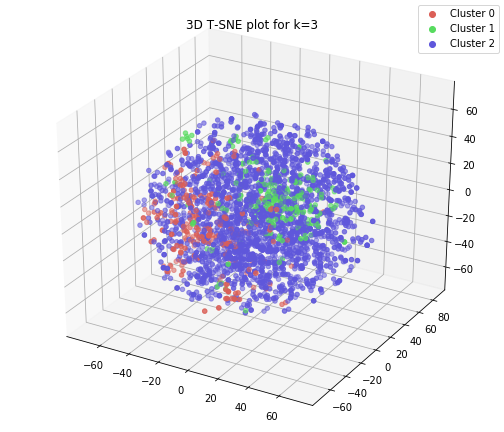
\includegraphics[width=0.45\textwidth]{images/kmeans_3d_tsne_k=3.png}\label{fig:ts3k3}}\\
	\caption{Decompositions of the clusters in 2 and 3 dimensions using PCA and T-SNE for k=3}
	\label{fig:k3pca}
\end{figure}
The Mahalanobis distance, as with the k=2, appear to be bimodal with a peak between 35 and 40, and a second peak above 50. The Euclidean distances are closer to being normally distributed. The majority of points are associated with cluster 2, with cluster 0 being the second biggest, and cluster 1 being the smallest.  


\begin{figure}[H]
	\centering
	\subfloat[Mahalanobis Distance]{  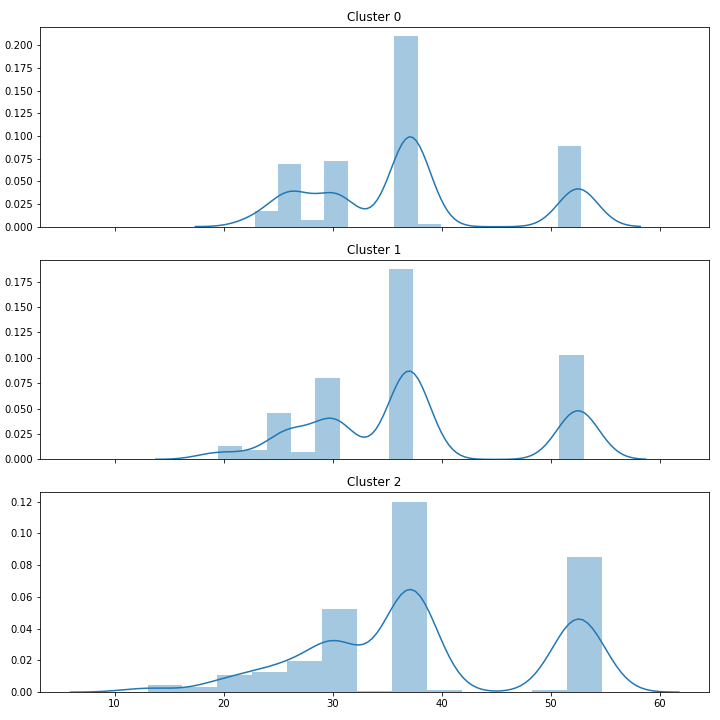
\includegraphics[width=0.45\textwidth]{images/kmeans_mahalanobis_distance_k=3.png}\label{fig:mhk3}}
	\subfloat[Euclidean Distances]{  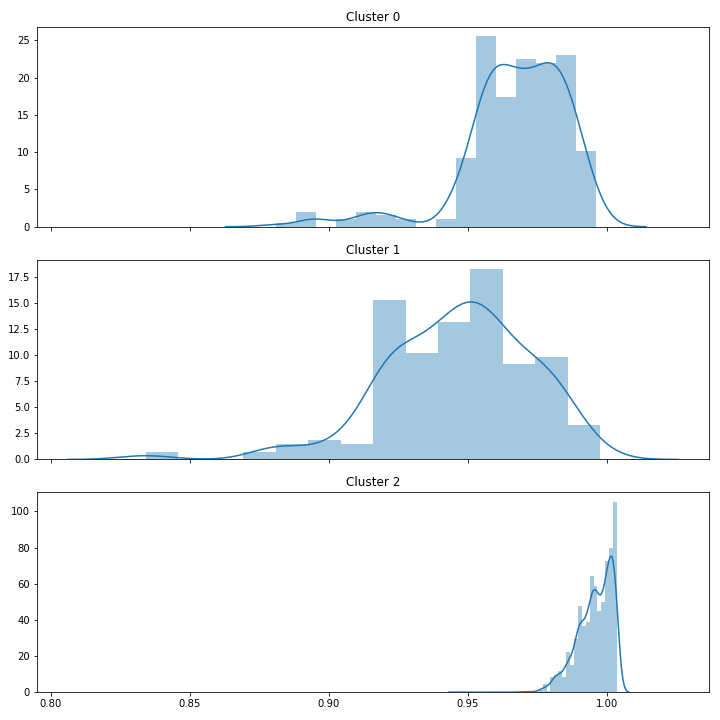
\includegraphics[width=0.45\textwidth]{images/kmeans_euclidean_distance_k=3.png}\label{fig:euk3}}\\
	
	\caption{Cluster Distances (Mahalanobis and Euclidean) for k=3 clusters}
	\label{fig:distk3}
\end{figure}

Comparing phrase distance with three clusters compared to two clusters, it is apparent that the distance behaviour is essentially similar in pattern with respect to both the distances from the clusters, and also the pattern of distances for the individual phrases, and the equality of the distances for each cluster.  
\begin{figure}[H]
	\centering
	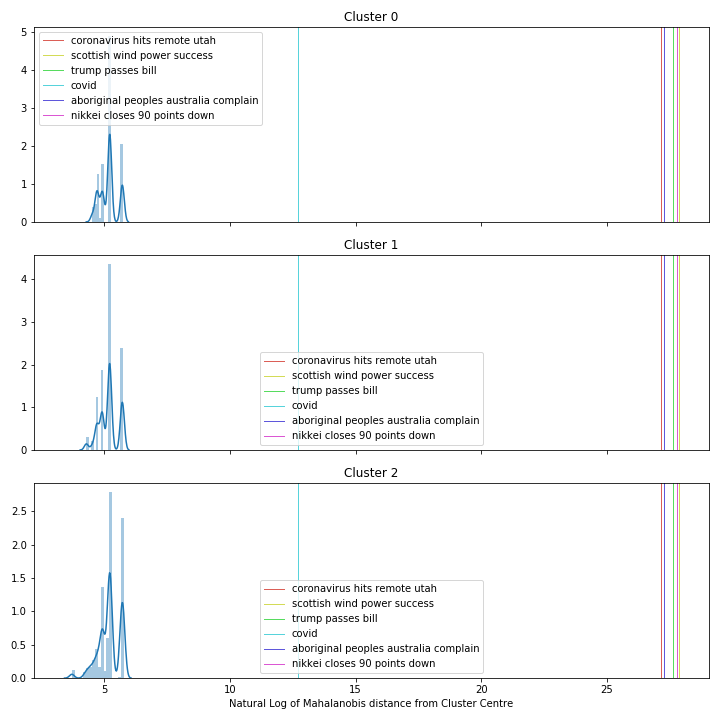
\includegraphics[width=0.8\textwidth]{images/words_kmeans_mahalanobis_distance_k=3.png}
	\caption{Log of Mahalanobis Distances for Clusters and Selected Phrases for k=3 clusters}
	\label{fig:wordsk3}
\end{figure}
\paragraph{Clustering when k=4}
Looking at the word clouds for 4 clusters It appears to be similar to both k=2 and k=3, in that all of the main words have been shared across the clusters. Cluster 2 has slightly more of the parsing errors associated with it, and thus is the more scattered of the clusters, and cluster 3 is slightly more focused on the pandemic in the US with words such as Test, and White House.

The decompositions are similar to the previous cluster results, especially in the PCA which suggests that boundaries between the clusters are very strong, but the `cluster` each cluster creates is not representative.
\begin{figure}[H]
	\centering
	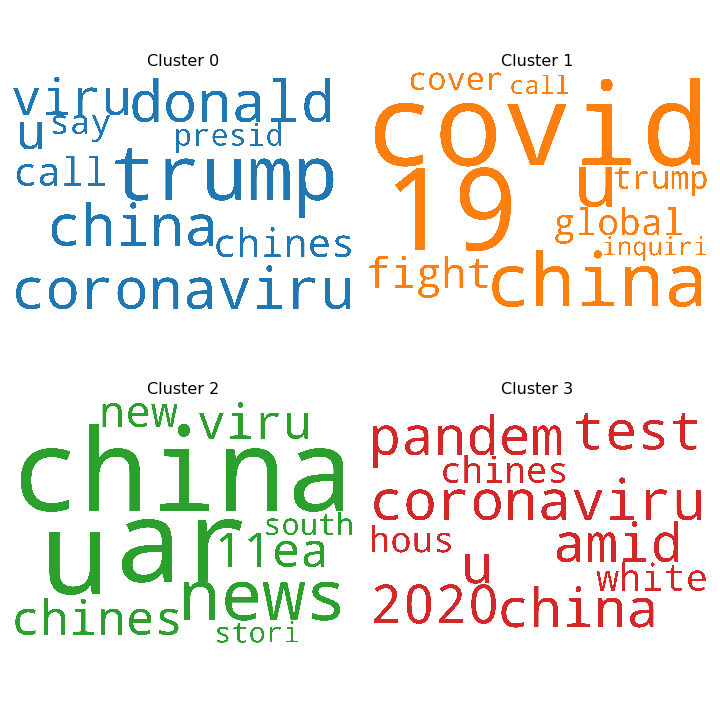
\includegraphics[width=0.8\textwidth]{images/kmeans_word_cloud_k=4.png}
	\caption{Word Cloud for k=4 clusters}
	\label{fig:wck4}
\end{figure}


\begin{figure}[H]
	\centering
	\subfloat[2D PCA k=4]{  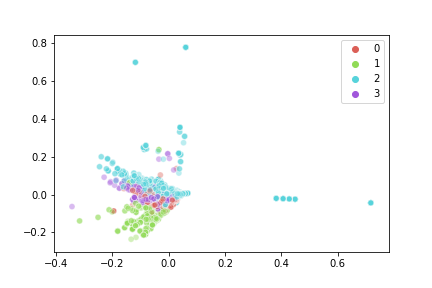
\includegraphics[width=0.45\textwidth]{images/kmeans_2d_pca_k=4.png}\label{fig:pca2k4}}
	\subfloat[3D PCA k=4]{  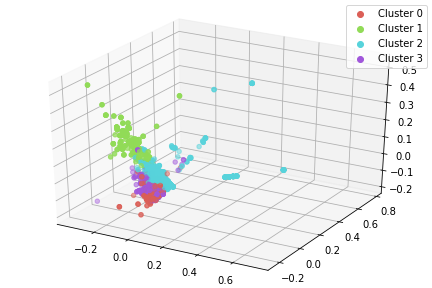
\includegraphics[width=0.45\textwidth]{images/kmeans_3d_pca_k=4.png}\label{fig:ts2k4}}\\
	\subfloat[2D T-SNE k=4]{  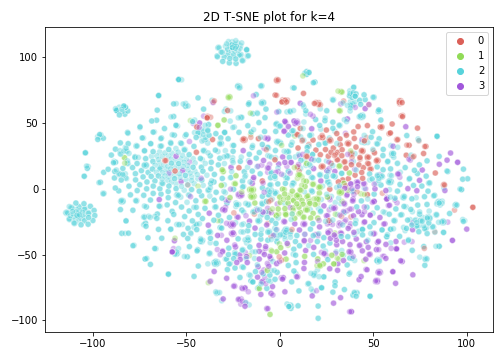
\includegraphics[width=0.45\textwidth]{images/kmeans_2d_tsne_k=4.png}\label{fig:pca3k4}}
	\subfloat[3D T-SNE k=4]{  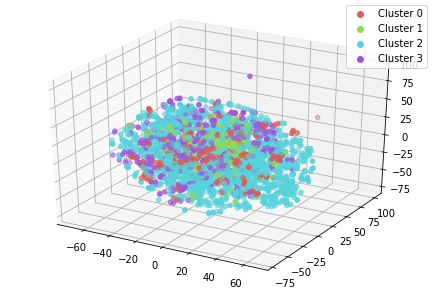
\includegraphics[width=0.45\textwidth]{images/kmeans_3d_tsne_k=4.png}\label{fig:ts3k4}}\\
	\caption{Decompositions of the clusters in 2 and 3 dimensions using PCA and T-SNE for k=4}
	\label{fig:k4pca}
\end{figure}
In line with the previous clusters, the Mahalanobis distance is also bimodal. The Euclidean distance as before appears to be more normal. In this cluster, Cluster 2 gets the majority of the words, followed by Cluster 3 and 0, and then Cluster 1. 

\begin{figure}[H]
	\centering
	\subfloat[Mahalanobis Distance]{  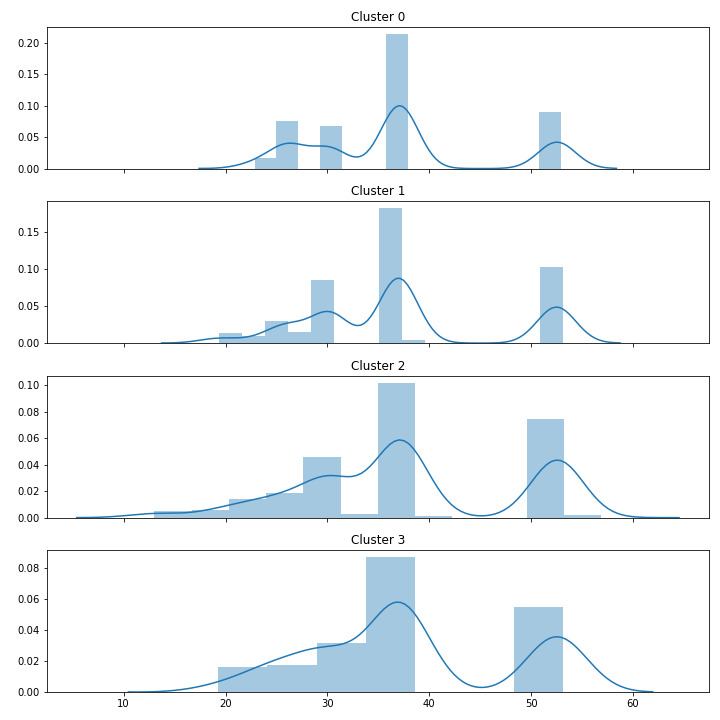
\includegraphics[width=0.45\textwidth]{images/kmeans_mahalanobis_distance_k=4.png}\label{fig:mhk4}}
	\subfloat[Euclidean Distances]{  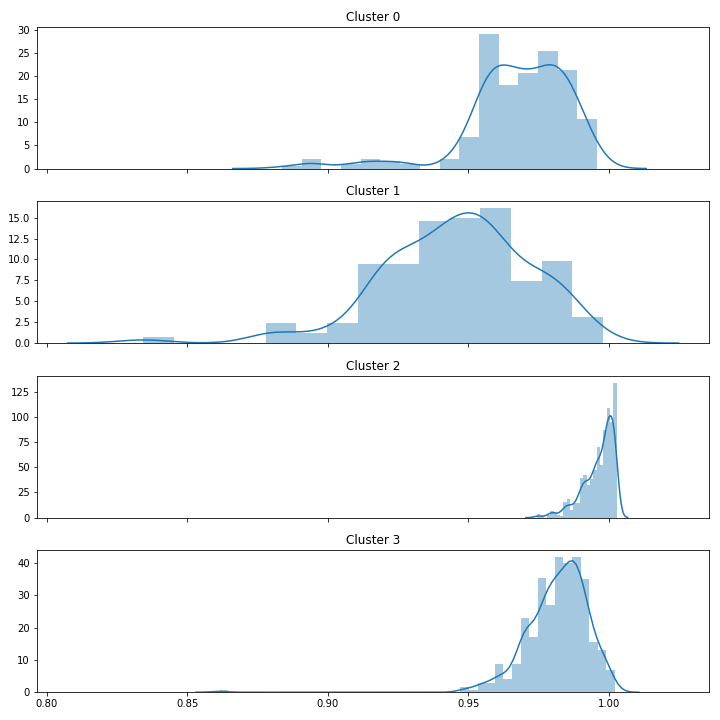
\includegraphics[width=0.45\textwidth]{images/kmeans_euclidean_distance_k=4.png}\label{fig:euk4}}\\
	
	\caption{Cluster Distances (Mahalanobis and Euclidean) for k=4 clusters}
	\label{fig:distk4}
\end{figure}

Comparing phrase distance with three clusters compared to both two and three clusters. The distance behaviour again appears to be identical across clusters, and the pattern of distances remains more or less the same. 
\begin{figure}[H]
	\centering
	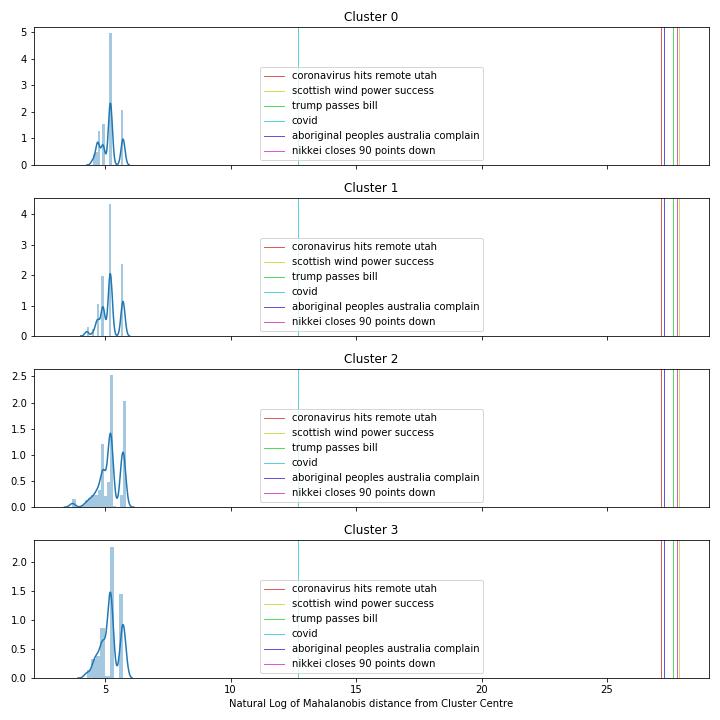
\includegraphics[width=0.8\textwidth]{images/words_kmeans_mahalanobis_distance_k=4.png}
	\caption{Log of Mahalanobis Distances for Clusters and Selected Phrases for k=4 clusters}
	\label{fig:wordsk4}
\end{figure}
\subsection{Modelling Stock Prices}
The table of accuracy predictions for the different models is shown in Table \ref{table:modaccuracy}. Several models had similar accuracy scores, though it should be noted that the predictions were on a very small dataset, so even one or two correct or incorrect predictions could sway the result considerably. 

The manually lagged models appeared to be the least best, in these models 5 days worth of previous days were added as 5 features to the data, and no other averaging methodology applied. Interestingly, the random forests classifiers appeared to do well with whatever data structure was used. Furthermore, models which applied moving window calculations did well, with on average the exponentially smoothed models doing the best.

With all of that taken into consideration, the best model was picked on the basis of being exponential and the random forests, and was found to be the exponential random forest.
\begin{table}[H]
	\centering 
\begin{tabular}{lr}

	Classifier &  Accuracy \\
	\hline
	Reference Classifier with Previous Day & 0.750\\
	\hline
                                  Naive Bayes &     0.750 \\
Logistic Regression &     0.750 \\
Averaged Random Forests &     0.750 \\
Gaussian Averaged Random Forests &     0.750 \\
Exponential Naive Bayes &     0.750 \\
Exponential Logistic Regression &     0.750 \\
Exponential Random Forests &     0.750 \\
Random Forests &     0.625 \\
Support Vector Machine &     0.625 \\
Averaged Naive Bayes &     0.625 \\
Averaged Logistic Regression &     0.625 \\
Averaged Support Vector Machine &     0.625 \\
Gaussian Averaged Naive Bayes &     0.625 \\
Gaussian Averaged Logistic Regression &     0.625 \\
Gaussian Averaged Support Vector Machine &     0.625 \\
Exponential Support Vector Machine &     0.625 \\
Manually 4 day lagged Random Forests &     0.625 \\
Neural Network & 0.500 \\
Manually 4 day lagged Naive Bayes &     0.500 \\
Manually 4 day lagged Logistic Regression &     0.500 \\
Manually 4 day lagged Support Vector Machine &     0.375 \\
	

\end{tabular}

	\caption{Table of Model Accuracy Results}
		\label{table:modaccuracy}
\end{table}

The best model's algorithm was used to train another model which just used the previous day's difference, as a reference to see if the model actually provided any improvement. It found that the accuracy improved considerably on the May June Data, with the reference model providing 50\% accuracy, and the exponentially smoothed random forest providing 62.5\% accuracy, which on the face of it is a significant improvement. 

The predictions are shown in figure \ref{fig:modelpred}, where the magnitude of the differences has been plotted, alongside whether the best model was correct in predicting a positive or negative shift (blanks are weekends or days when the stock market didn't operate). There does not appear to be a time based prediction component, the model is just as likely to predict correctly or incorrectly regardless of the time that it is predicting on. Interestingly, the model does not appear to be very good at predicting for large stretches correctly, it correctly predicts for a day or two, and then has incorrect predictions for a similar length of interval. The exception to this is when halfway through the prediction, the model correctly predicts the spike and the subsequent fall and recovery. 

The distribution of magnitude of the positive and negative daily differences is plotted in Figure \ref{fig:distmodel}.  It is apparent that the model is better at predicting smaller differences in the stock market. the majority of incorrect predictions come from larger negative values and slightly from the positive jumps. There are significantly fewer incorrect predictions when the market jumps between -500 and +500 points. Interestingly, there is a small bump at a large positive value of +1000, suggesting the model was good at predicting large positive values. 

\begin{figure}[H]
	\centering
	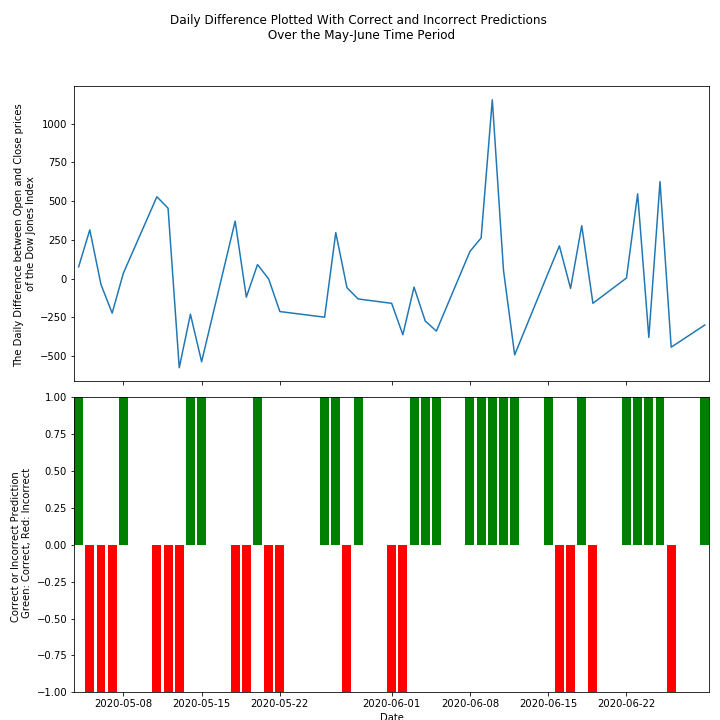
\includegraphics[width=0.8\textwidth]{images/model_pred_time.png}
	\caption{The Dow Jones daily changes in prediction dataset, and whether the model predicted the the result correctly or not)}
	\label{fig:modelpred}
\end{figure}


\begin{figure}[H]
	\centering
	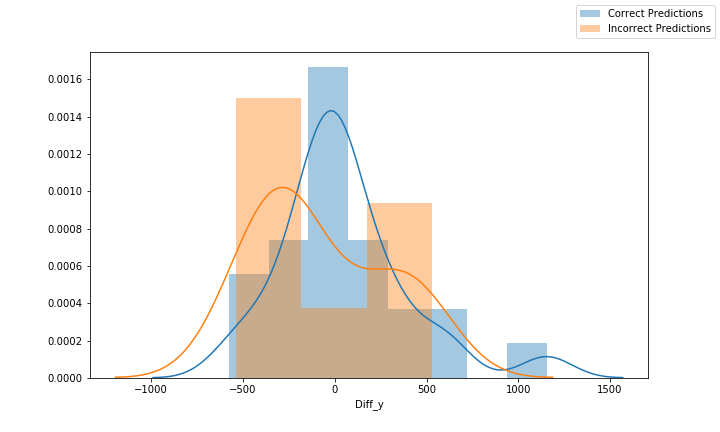
\includegraphics[width=0.8\textwidth]{images/dist_of_model.png}
	\caption{The distribution of the daily differences between open and close prices where the model predicted correctly vs predicted incorrectly)}
	\label{fig:distmodel}
\end{figure}





